%Preamble
\documentclass[12pt]{article}
\usepackage[utf8]{inputenc}
\usepackage{graphicx}
\usepackage{url}
\usepackage{setspace}
\usepackage{float}
\usepackage{siunitx}
\usepackage[ngerman]{babel}
\usepackage[version=4]{mhchem}
\setstretch{1.5}
\usepackage{geometry}
\geometry{a4paper, portrait, margin=30mm, bmargin=30mm, tmargin=30mm}
\usepackage{amsmath}

%Bibliography
%\usepackage[backend = biber, style = alphabetic, sorting = ynt]{biblatex}
%\addbibresource{thesis.bib}
\bibliographystyle{unsrt}

%Patch abstract command to make it normal size
\makeatletter
\renewenvironment{abstract}{%
    \if@twocolumn
      \section*{\abstractname}%
    \else %% <- here I've removed \small
      \begin{center}%
        {\bfseries \Large\abstractname\vspace{\z@}}%  %% <- here I've added \Large
      \end{center}%
      \quotation
    \fi}
    {\if@twocolumn\else\endquotation\fi}
\makeatother


\begin{document}
\begin{center}
\thispagestyle{empty}
\large{\textbf{University of Innsbruck}}\\[-0.9ex]
\large{Department of General, Inorganic and Theoretical Chemistry}\\
\vspace{0.3cm}
\begin{center}

\includegraphics[width=7cm]{Images/Logo.jpg}\\
\vspace{0.9cm}
\textbf{\LARGE{Laborprotokoll}}\\
\medskip\par
\vspace{1.2cm}
\Large{\textbf{Anorganisch-chemisches Praktikum für Fortgeschrittene}}\\[-0.5ex]
\vspace*{1.5cm}
\bigskip\par
\textbf{Michael Helmut Fill, BSc. }\\[-1ex]
11704837\\
\vspace*{1.5cm}
\textbf{Betreuung:} \\ Mag. Ingo Widmann, MSc \\ Dr. Stefan Schwarzmüller\\

\bigskip \par

\small{\textbf{Durchführung:} \\ 13.05.2024 - 28.05.2024\\}

\small{\textbf{Abgabe:} \\ 10.6.2024\\}
\small{\textbf{Abgabe der Korrektur:} \\ 23.6.2024\\}
\end{center}
\end{center}

\newpage

\tableofcontents

\newpage

\section{Einleitung}
Verschiedene Methoden aus dem Bereich der Festkörperchemie wurden in einem zweiwöchigen Praktikum zur Synthese spezialisierter Feststoffe angewendet.
Zum einen wurden Experimente in der Hochdruckpresse bzw.~im Hochofen durchgeführt um metastabile Phasen von \ce{CuSb3Se5}, \ce{LiMoS2} und \ce{GaB4O6N} herzustellen.
Synthesen unter Hochdruckbedingungen sind vor allem in industriellen Verfahren etabliert, da dort der finanzielle Aufwand für Geräte und Energie durch die massiv erhöhten Reaktionsgeschwindigkeiten und Ausbeuten ausgeglichen wird. 
Das seit den Anfängen des 20. Jahrhunderts großtechnisch relevante, nach Fritz Haber und Carl Bosch benannte, Haber-Bosch-Verfahren zur Ammoniaksynthese ist hierbei wohl eines der bekanntesten und ältesten Beispiele der Hochdruckchemie, bei welchem mit Drücken von bis zu 350 bar und Temperaturen von bis 500 \si{\degreeCelsius} gearbeitet wird~\cite{Timm1963}.
Wo heute Syntheseanlagen mit modernen Turbokompressoren ausgestattet sind findet sich im originalen Schema von Fritz Haber eine Umlaufpumpe, also ein stehender einstufiger Hubkolbenverdichter~\cite{deutscheschemiemuseumUmlaufpumpe}.
Ein weiterer Durchbruch im Bereich der Hochdrucksynthese gelang 1954 mit der ersten kommerziell erfolgreichen Synthese eines Diamanten nach dem \textit{High-Pressure High-Temperature} (HPHT) Verfahren, bei welchem Graphit unter Drücken von über 10 GPa und Temperaturen von 2000 \si{\degreeCelsius} in Diamant umgewandelt wird.
Zur Druckerzeugung wurde hierbei eine Bandpresse  eingesetzt, bei der ein Ring aus gehärtetem Stahl auf die Belastungsgrenze gedehnt und um die Probe gewickelt wird~\cite{Hall1960}.
Über die nächsten Jahrzehnte folgten weitere Entwicklungen des HPHT Verfahrens, wie die im Praktikum verwendete Multianvil-Hochdruckpresse oder hocheffiziente Spaltkugelpressen (BARS)~\cite{Abbaschian2005}.
Zusätzlich wurden fünf unterschiedliche Hydrothermalansätze in Autoklaven durchgeführt, bei denen Ammoniumfluorid und Borsäure zusammen mit verschiedenen Aluminium- bzw.~Galliumnitraten und -oxiden verwendet wurden.
Autoklavenansätze beziehen sich in der anorganischen Chemie vor allem auf Solvothermalsynthesen, wo gelöste Edukte unter Druck und hohen Temperaturen zur Reaktion gebracht werden sollen~\cite{Rabenau1985}. Weitere Anwendungsgebiete für Autoklaven sind die großtechnische Überführung von Kautschuk in elastomere Gummis (Vulkanisation) oder die Herstellung thermoplastischer Kunststoffe wie Polyethylen.
Die Analyse der wie beschrieben erhaltenen Produkte erfolgte über Röntgenpulverdiffraktometrie, deren Ergebnisse mit Werten aus der bekannten Literatur und Simulationsdaten verglichen wurden.
Zusätzlich wurden neben der Analyse der genannten Ansätze verschiedene Substanzen im Rahmen einer theoretischen Einführung \textit{via} Rasterelektronenmikroskopie untersucht, wobei hierbei keine für dieses Praktikum relevanten Daten extrahiert wurden.
Neben den genannten Methoden wurden auch die Grundlagen verschiedener in der anorganischen Chemie relevanter Softwareprogramme erläutert sowie einfache Glasbearbeitungen und Arbeiten in der Glovebox durchgeführt.
\subsection{Urheberrechtlicher Hinweis}
Alle im Rahmen dieses Protokolls verwendeten Fotos wurden entweder einvernehmlich von Kommilitonen erhalten und in den Bildunterschriften mit dem Urheber gekennzeichnet oder stammen aus eigener Hand.
\section{Methoden}
\subsection{Experimentelle Methoden}
\subsubsection{Multianvil-Hochdruckpresse}
Die verschiedenen Hochdrucksynthesen wurden an der \textit{mavo press} LPR 1000-400/50 Hochdruckpresse, hergestellt durch die Max Voggenreiter GmbH, durchgeführt~\cite{Voggenreiter}.
Hierbei wird der Druck hydraulisch mittels Öl aufgebaut, welcher uniaxial auf das sogenannte Walker-Type Modul, einem dicken, wasserkühlbaren Stahlgefäß mit 6 Stahlkeilen, übertragen wird. Die Presse und das Walker-Type Modul sind in den Abbildungen \ref{fig:pressepresse} und \ref{fig:walkerwalker} dargestellt. 
In diesem Modul wird daraufhin der Druck auf die achtteiligen Wolframcarbidwürfel übertragen, in welchem die Probensubstanz komprimiert wird, wobei darauf geachtet werden muss, das Walker-Type Modul und die Stahlkeile mit isolierender PET-Folie zu ummanteln.

\begin{figure}[H]
    \centering
    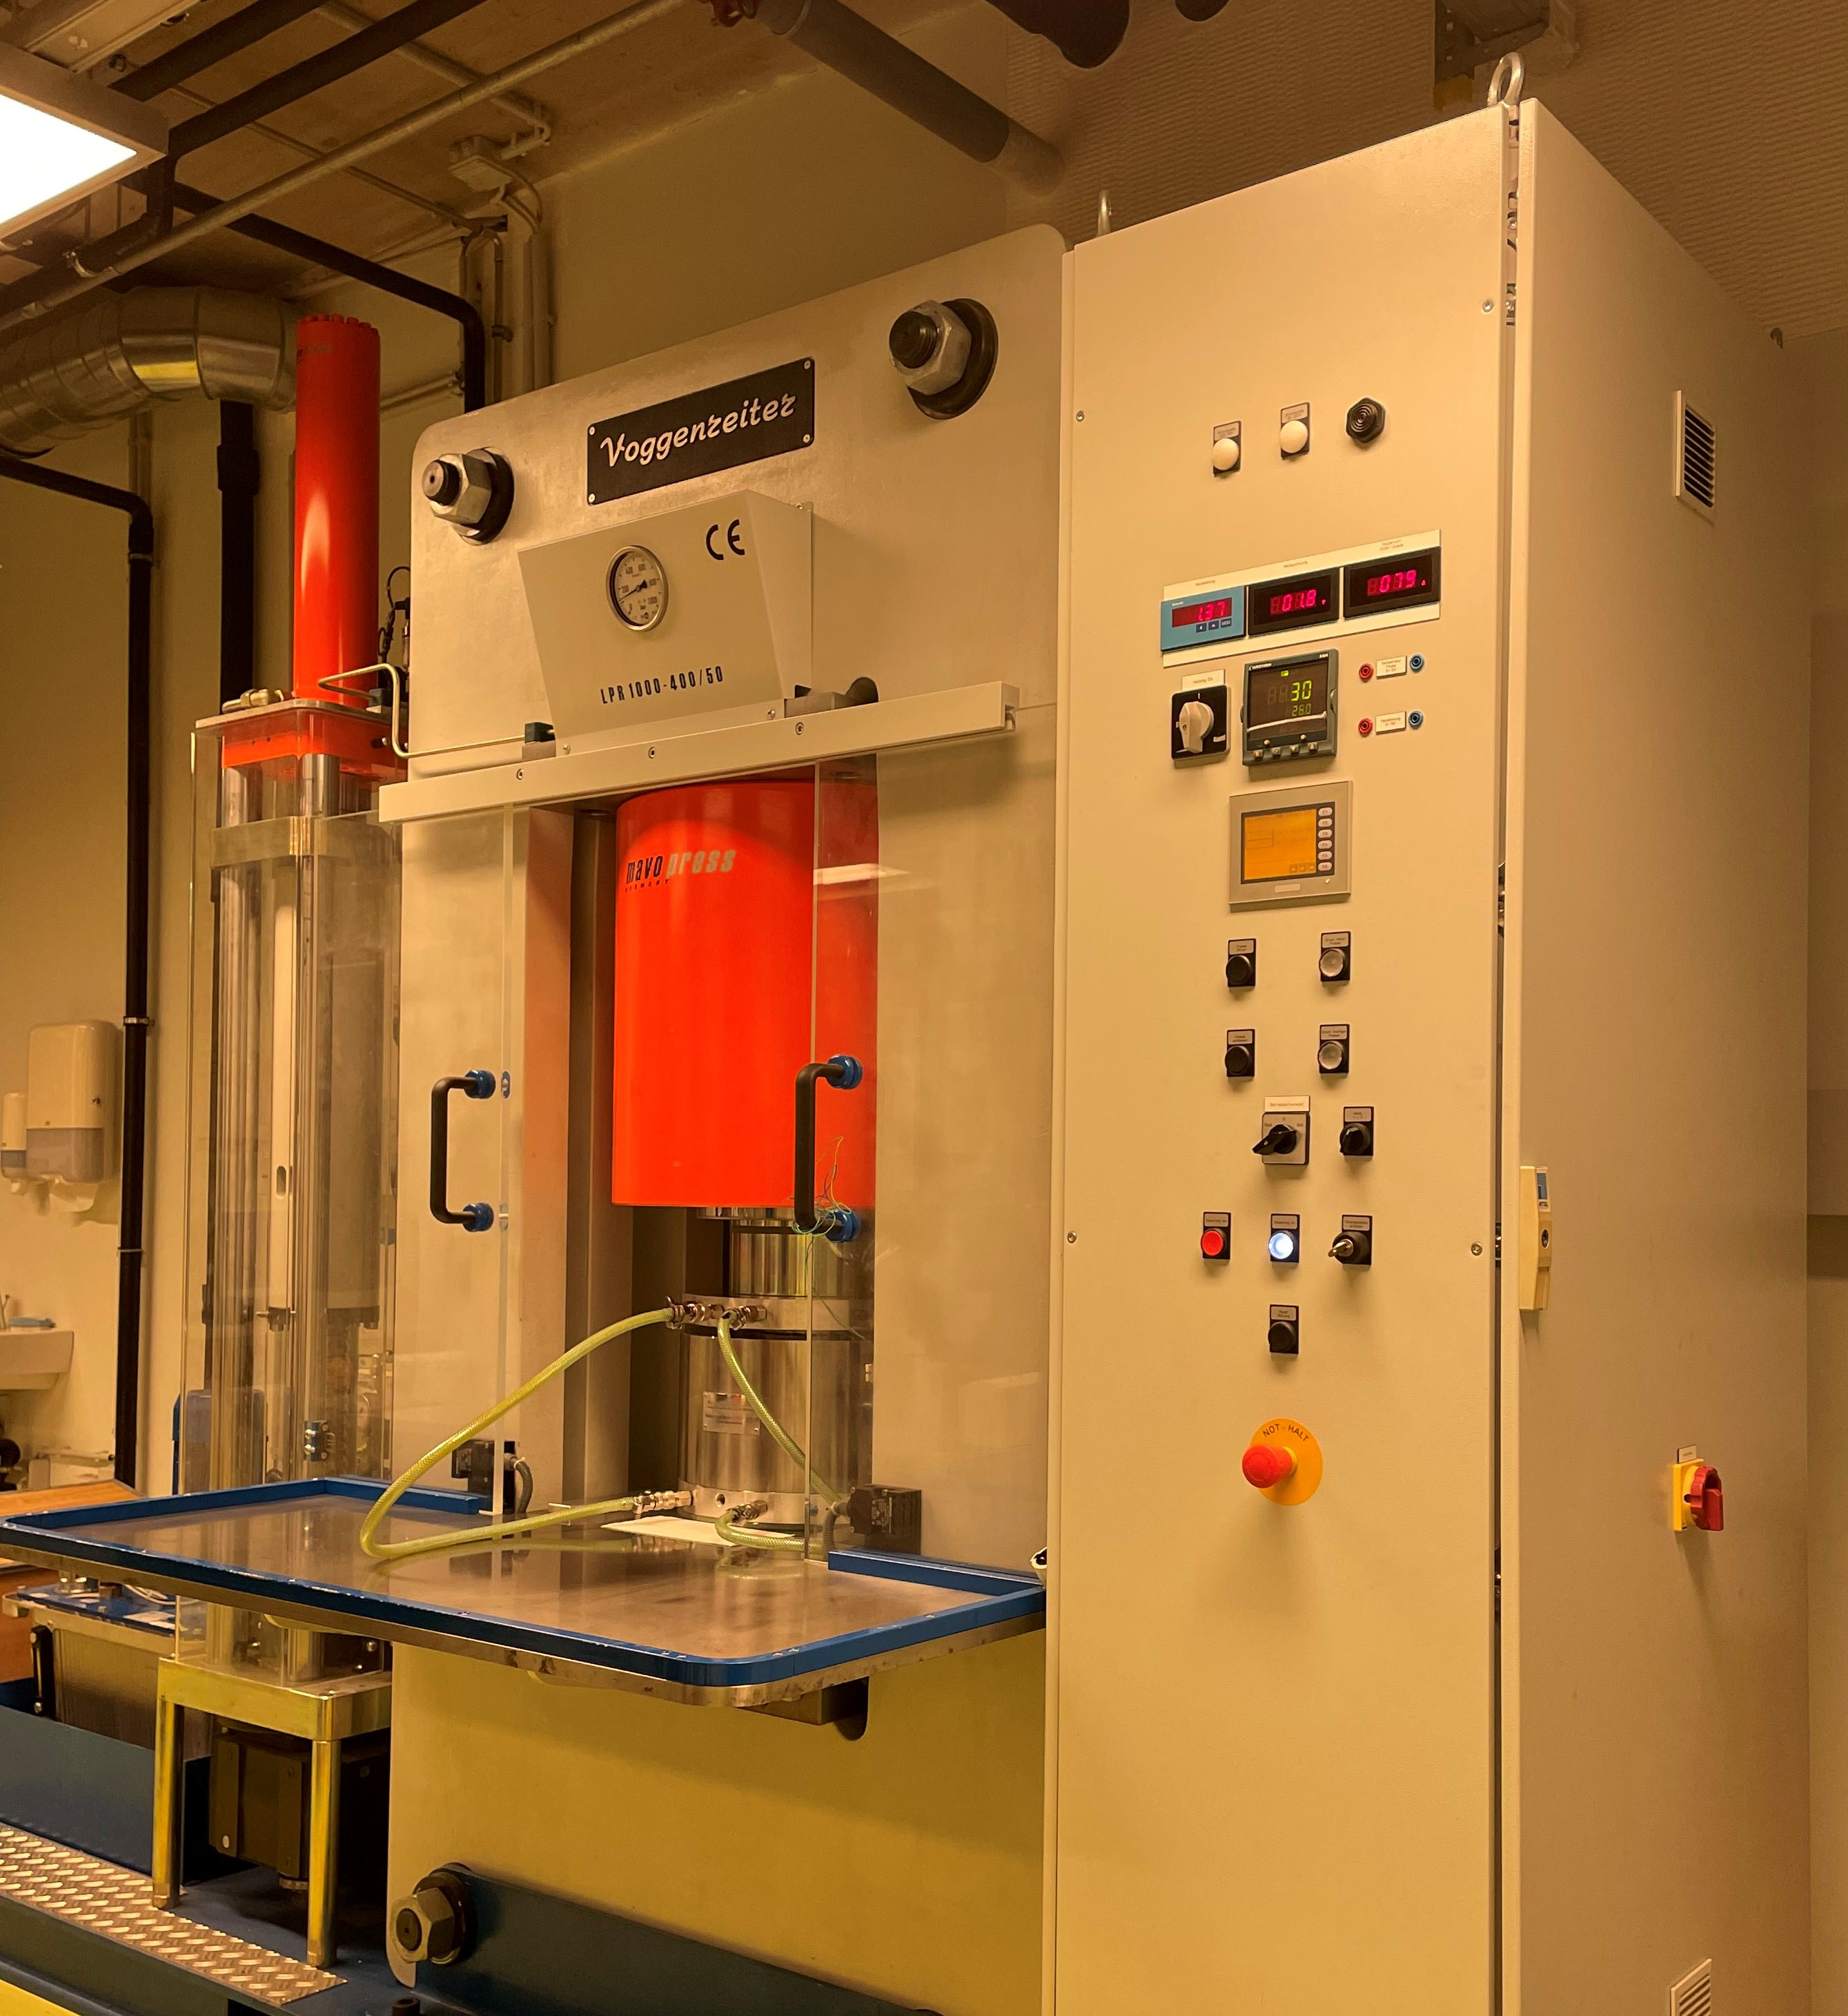
\includegraphics[height=8cm]{Images/Presse.jpg}
    \caption{\textit{mavo press} LPR 1000-400/50 Hochdruckpresse. Bildurheberin: Sabine Lerch, BSc.}
    \label{fig:pressepresse}
\end{figure}
\begin{figure}[H]
    \centering
    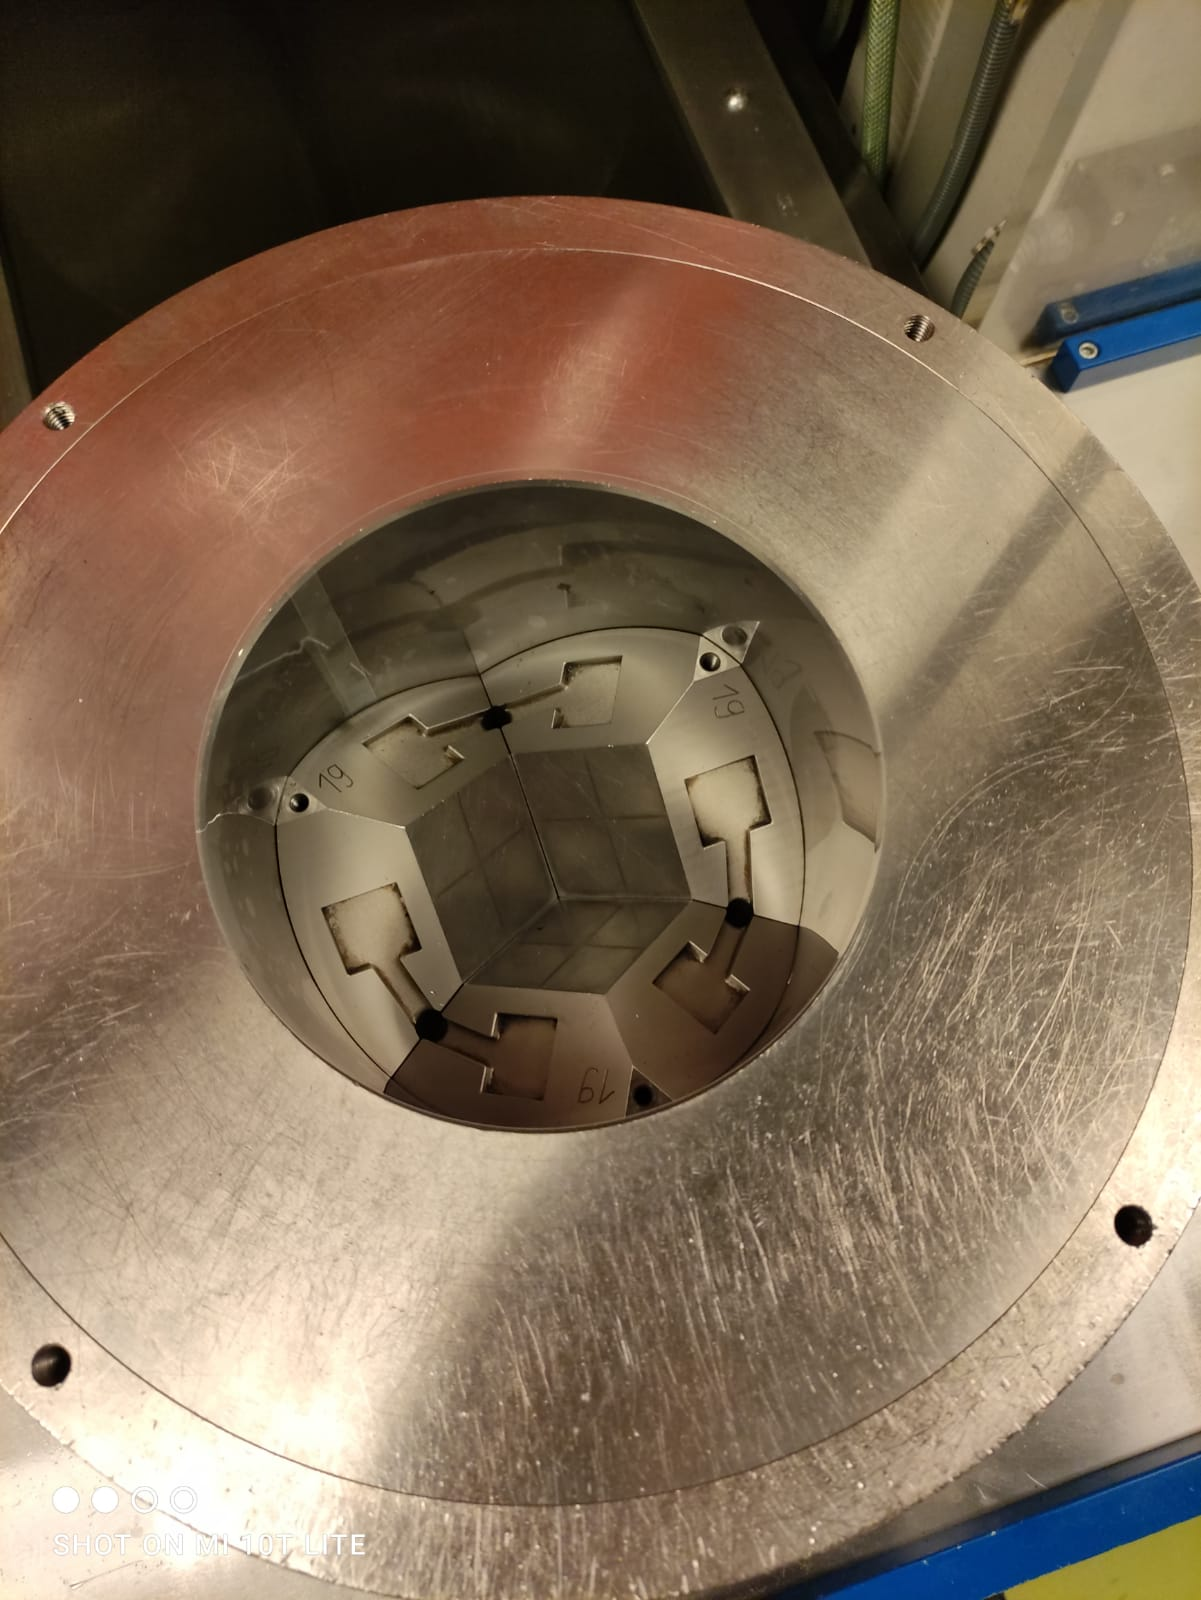
\includegraphics[height=8cm]{Images/Walker.jpeg}
    \caption{Offenes Walker-Type Modul mit den drei unteren der insgesamt sechs Stahlkeile. Bildurheberin: Sabine Lerch, BSc.}
    \label{fig:walkerwalker}
\end{figure}

\subsubsection{Probenvorbereitung im Hochdruckverfahren}
Die Proben der Hochdruckansätze wurden in 18/11 bzw. 14/8 Assemblies vorbereitet, wobei die erste Zahl für die Kantenlänge des verwendeten Oktaeders und die zweite für die Kantenlänge der abgeschnittenen Ecken der Wolframcarbid Würfel, jeweils in mm, steht. 
Die fein gemörserten Precursor werden in einen Tiegel aus hexagonalem Bornitrid gepackt, welcher danach vorsichtig in einen kleinen Graphitofen eingesetzt wird.
Dieser wird mit einem Bornitrid-Deckel verschlossen und in einen größeren \ce{ZrO2} Graphitofen verpackt, welcher beidseitig mit \ce{MgO}-Spacern zur Zentrierung im Okteader versehen wird.
Dieser Zylinder wird schlussendlich in ein \ce{MgO}-Oktaeder (5\% \ce{Cr2O3}) eingesetzt und an beiden Enden mit leitenden Molybdänplättchen versehen, bevor der gesamte Aufbau im Zentrum der acht Wolframcarbidwürfeln platziert wird. Die Heizung erfolgt elektrisch über die Molybdänplättchen und Graphitöfen, wobei letztere bei Anlegen einer Spannung durch den elektrischen Widerstand von Graphit erhitzt werden.
Abbildung \ref{fig:14-8} zeigt die oben genannten Bauteile für ein 14/8 Assembly, welches sich vom 18/11 Assembly nur durch die geringere Größe und die zwei zusätzlichen \ce{MgO} Abstandsringe unterscheidet.
\begin{figure}[H]
    \centering
    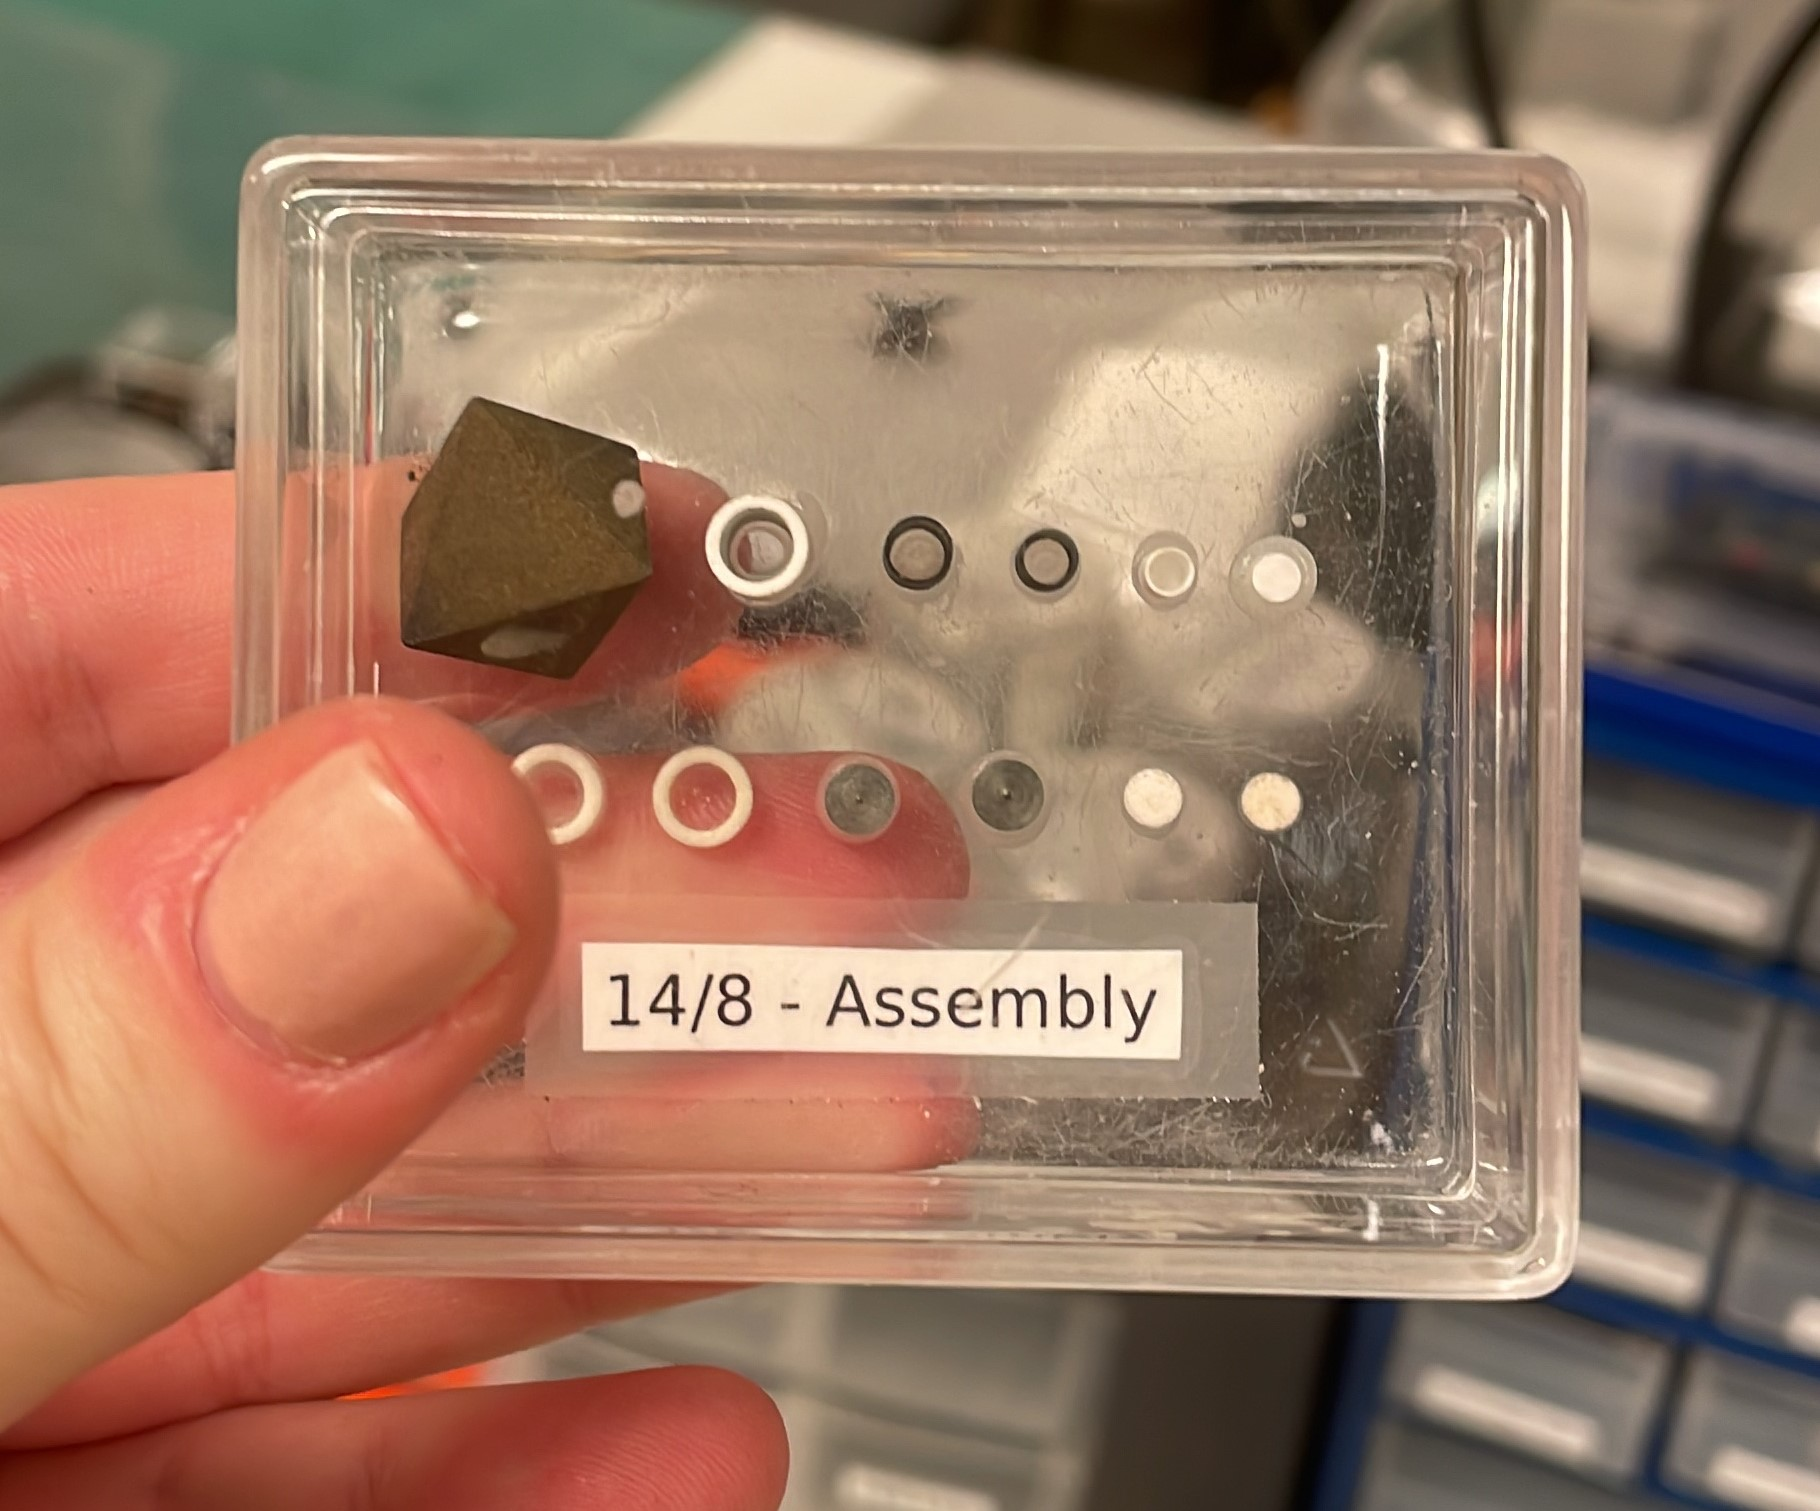
\includegraphics[height=8cm]{Images/14-8.jpg}
    \caption{14/8 Assembly, welches sich vom 18/11 Assembly nur durch die geringere Größe und die zwei zusätzlichen \ce{MgO} Abstandsringe unterscheidet. \\Bildurheberin: Sabine Lerch, BSc.}  
    \label{fig:14-8}
\end{figure}

\noindent Um den Abstand zum Oktader zu wahren und um zu verhindern, dass das Oktaeder zwischen die Würfel gepresst wird, wurden vier der acht Würfel um die Kontaktfläche mit Pyrophilitdichtungen abgeklebt. Zusätzliche Kartonplättchen hinter den Dichtungen sowie Teflonbandbeschichten auf den restlichen vier Würfeln sollen das Ausfließen dieser Dichtungen verhindern bzw. verzögern.
Die Würfel werden dann auf allen sechs Seiten von glasfaserverstärkten Kunststoffplatten umgeben, wobei nur die unterste und oberste Platte zur Stromleitung zusätzlich mit einem kleinen Stück Kupferblech versehen werden.
Die Abbildungen \ref{fig:würfel1} bis \ref{fig:würfel4} zeigen verschiedene Stufen des Aufbaus, beginnend mit den unteren vier WC-Würfeln bis zum vollständigen Würfel im Walker-Type Modul.

\begin{figure}[H]
    \centering
    \includegraphics[height=8cm]{Images/Würfel1.jpeg}
    \caption{18/11 Assembly mit den unteren vier WC-Würfeln. Zwei der vier Würfel wurden mit Teflonband beklebt, die anderen beiden mit Pyrophilitdichtungen und Karton abgeklebt. Hierbei ist darauf zu achten, den mit dem Molybdänplättchen in Kontakt stehenden Würfel zu markieren.}
    \label{fig:würfel1}
\end{figure}

\begin{figure}[H]
    \centering
    \includegraphics[height=8cm]{Images/Würfel2.jpeg}
    \caption{18/11 Assembly mit sieben der acht WC-Würfel. Der letzte einzusetzende Würfel steht in Kontakt mit dem hier erkennbaren Molybdänplättchen.}
    \label{fig:würfel2}
\end{figure}

\begin{figure}[H]
    \centering
    \includegraphics[height=8cm]{Images/Würfel3.jpeg}
    \caption{Vollständiger Würfel bei dem die obere Kupferblechplatte mit dem leitenden Wolframcarbidwürfel in Kontakt steht.}
    \label{fig:würfel3}
\end{figure}

\begin{figure}[H]
    \centering
    \includegraphics[height=8cm]{Images/Würfel4.jpeg}
    \caption{Vollständiger Würfel, eingesetzt in die unteren Stahlkeile des Walker-Type Moduls.}
    \label{fig:würfel4}
\end{figure}

\subsubsection{Muffelofen}
Einer der Ansätze im Laufe des Praktikums wurde im L 5/13 Muffelofen der Firma Nabertherm durchgeführt, zu sehen in Abbildung \ref{fig:ofenmuffi}. Dieser besteht aus einem Gehäuse aus Edelstahl und internen Hochofenziegelisolierungen, wobei die Heizelemente direkt im Inneren des Ofens angebracht sind.
Dieser Ofen ist in der Lage, eine Maximaltemperatur von 1300 \si{\degreeCelsius} zu erreichen, wobei die Temperatur über einen digitalen Regler eingestellt und über einen Thermoelementfühler gemessen wird.~\cite{Nabertherm}

\begin{figure}[H]
    \centering
    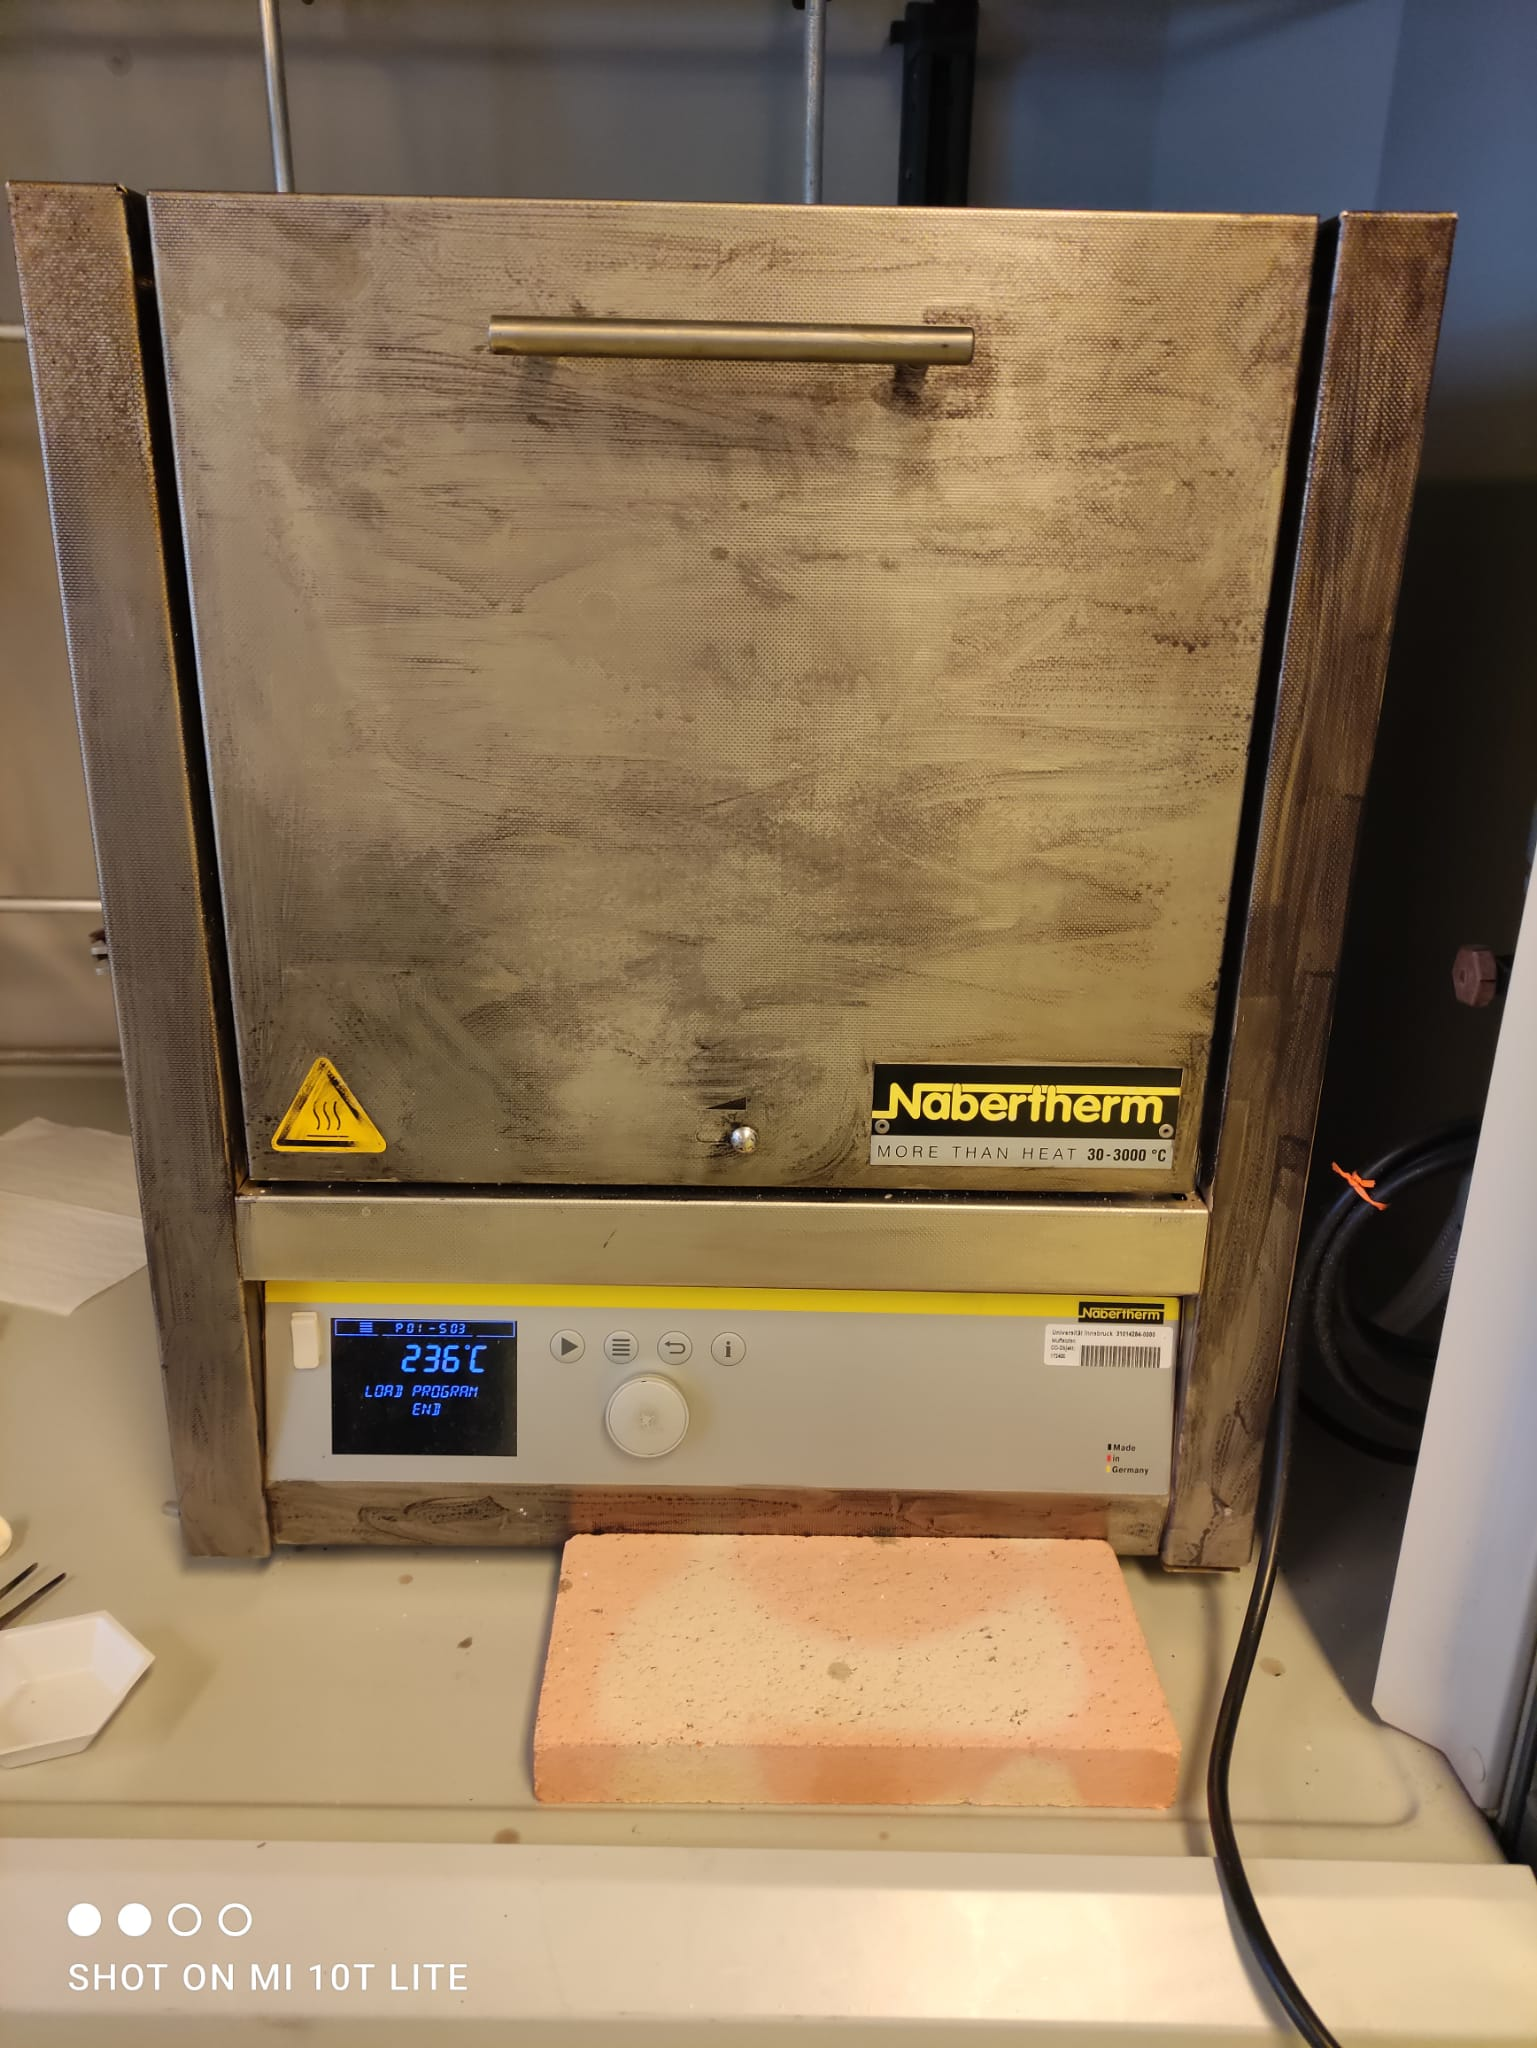
\includegraphics[height=8cm]{Images/Ofen.jpeg}
    \caption{Nabertherm L 5/13 Muffelofen.}
    \label{fig:ofenmuffi}
\end{figure}

\subsubsection{Autoklavenansatz im Konvektionsofen}
Die Hydrothermalansätze wurden in Autoklaven im Konvektionsofen der Firma Thermo Scientific, zu sehen in Abbildung \ref{fig:ofenauto}, durchgeführt~\cite{thermofisherHerathermGeneral}.
Nach Einwaage der Precursor und Solvatation in Wasser wurden die Lösungen in die vorher gereinigten Autoklaven gegeben und daraufhin bis zu 24 Stunden in verschiedenen Temperaturbereichen behandelt.
Abb. \ref{fig:klavori} zeigt einen der verwendeten Autoklaven.

\begin{figure}[H]
    \centering
    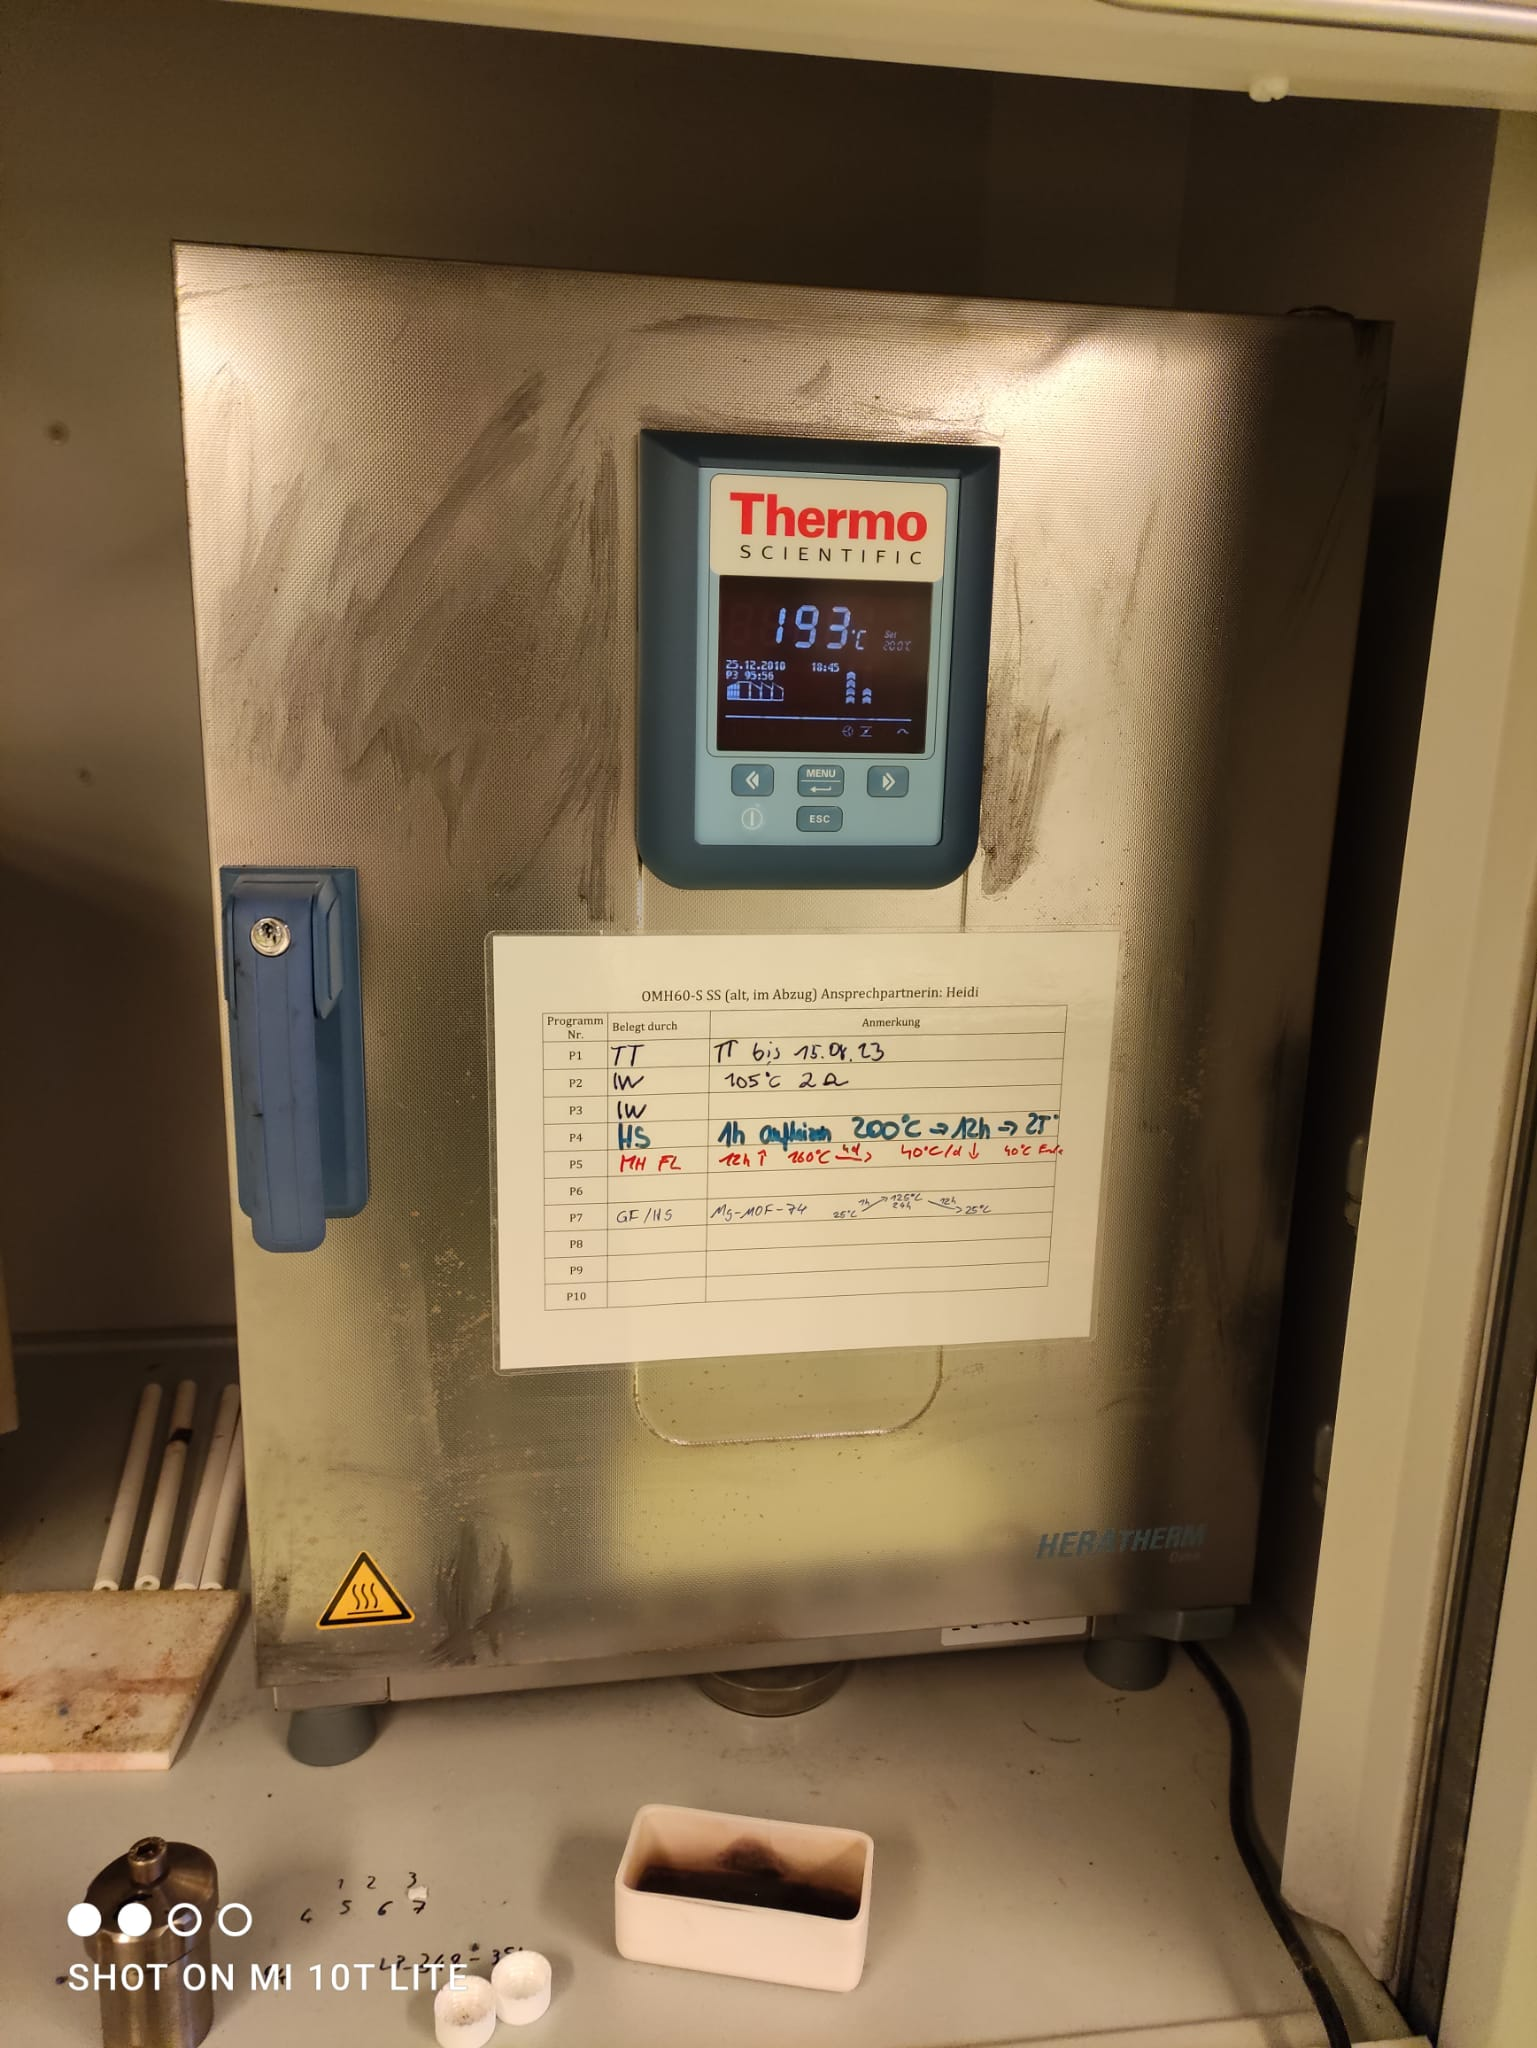
\includegraphics[height=8cm]{Images/Konvektionsofen.jpeg}
    \caption{Konvektionsofen der Firma Thermo Scientific.}
    \label{fig:ofenauto}
\end{figure}

\begin{figure}[H]
    \centering
    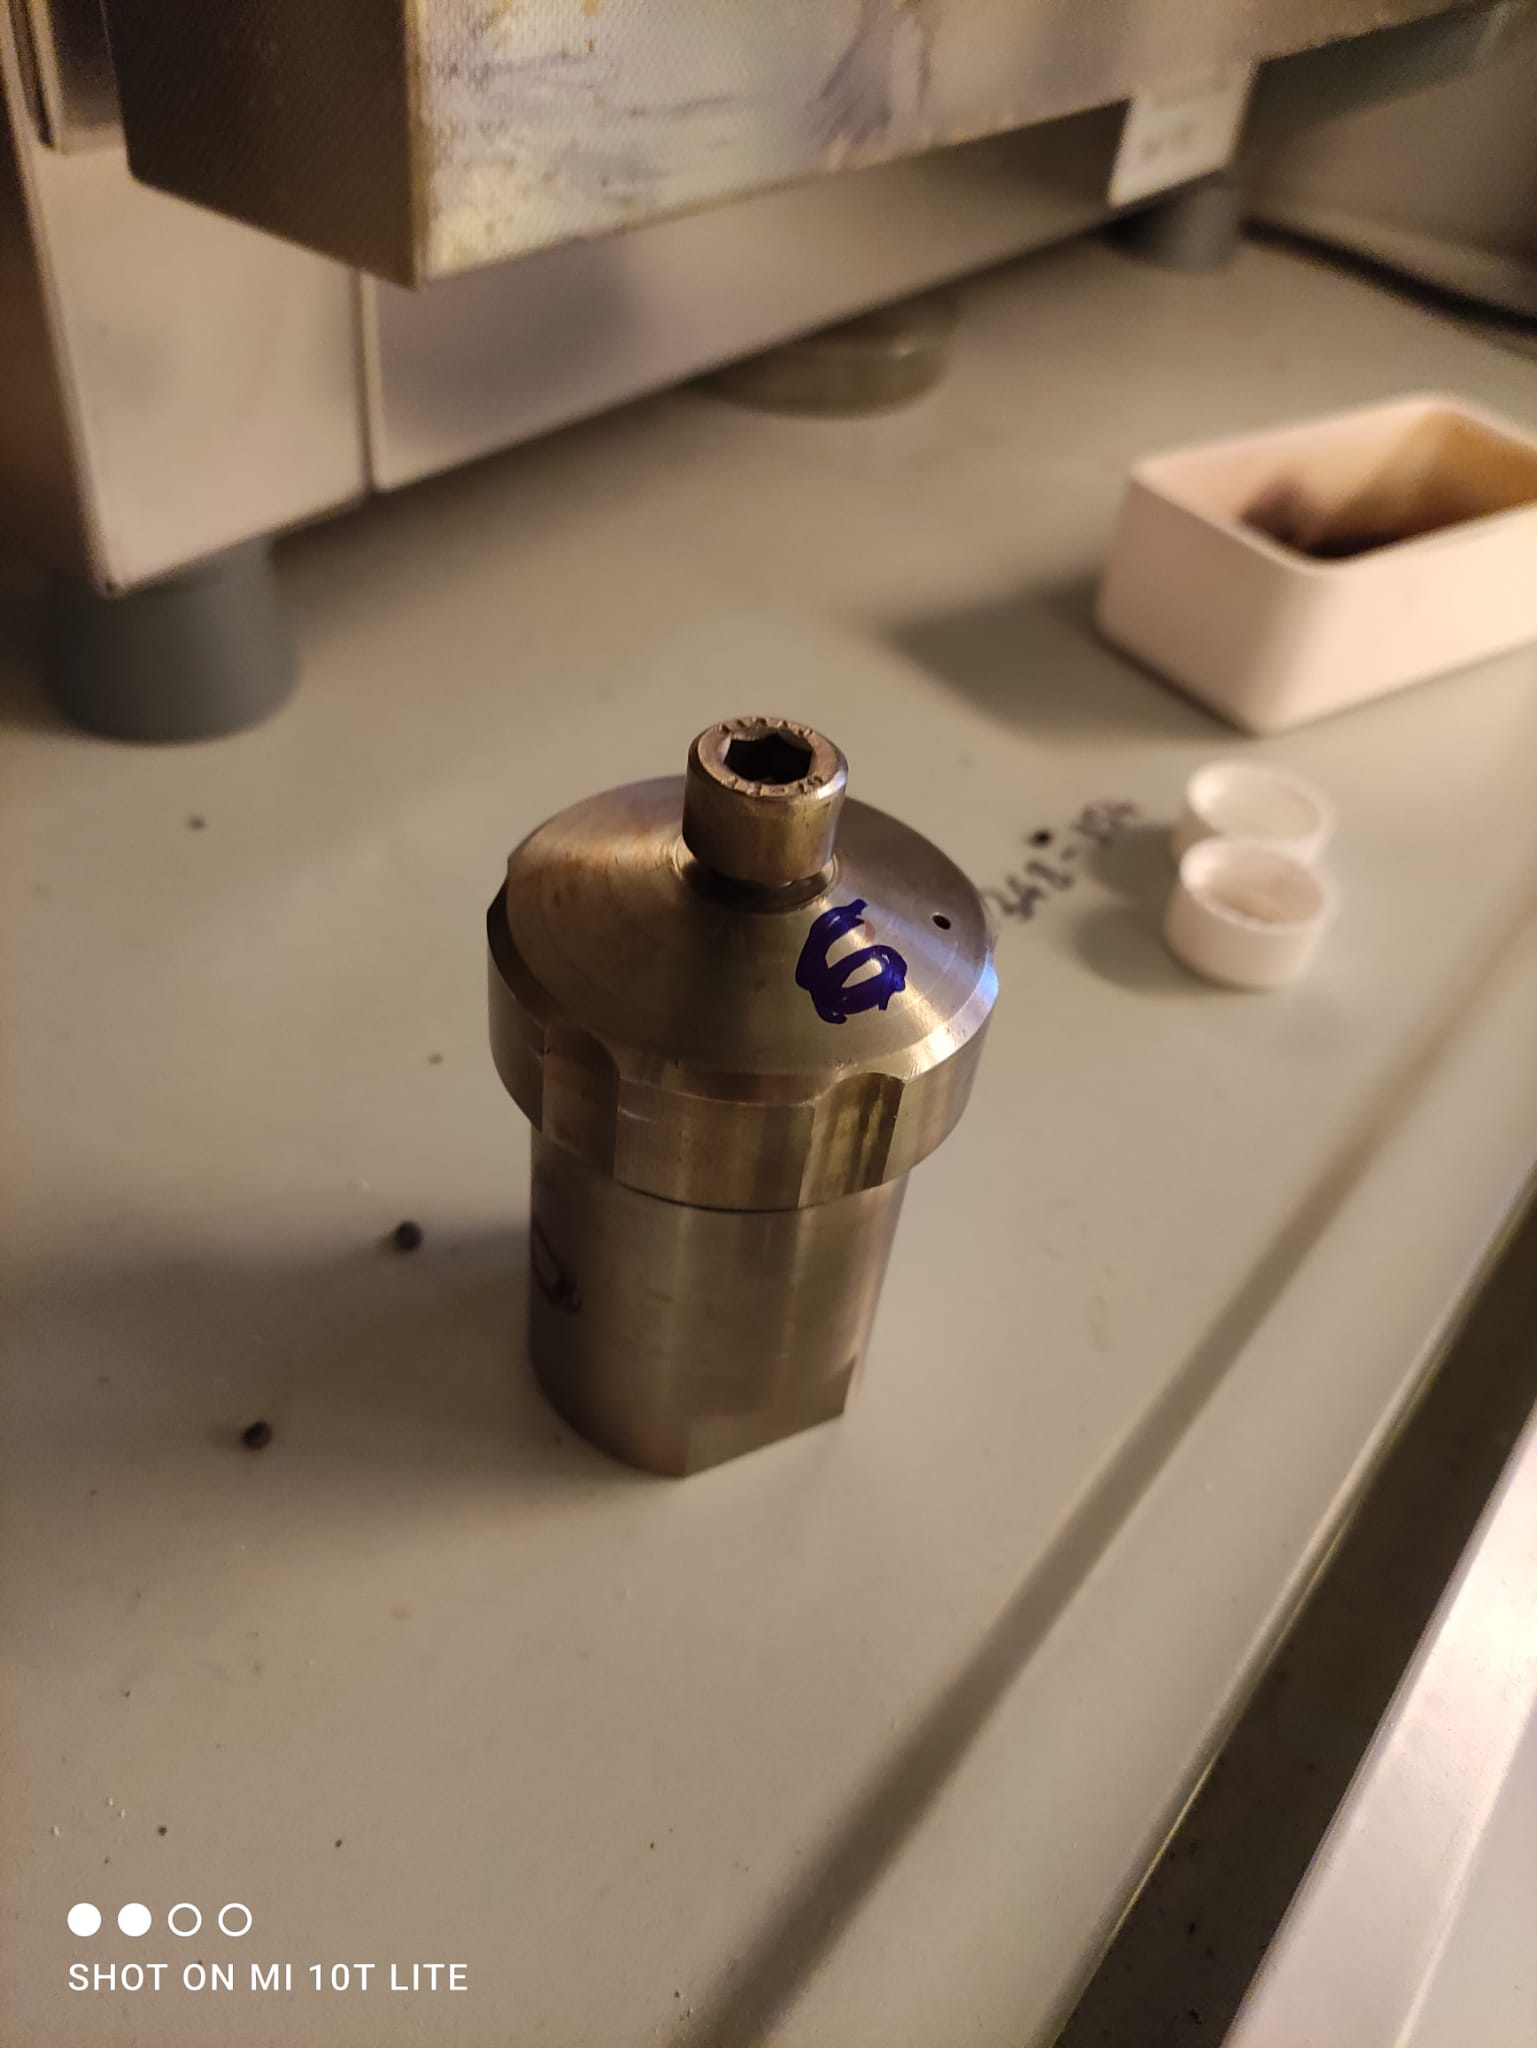
\includegraphics[height=8cm]{Images/Autoklave.jpeg}
    \caption{Einer der für das Hydrothermalverfahren verwendeten Autoklaven.}
    \label{fig:klavori}
\end{figure}



\subsubsection{Glasbearbeitung}
Um Nebenreaktionen und Verunreinigungen bei Normaldrucksynthesen zu vermeiden wurden bei manchen Ansätzen die Precursor in Glasampullen gefüllt und unter Luft- und Feuchtigkeitsausschluss in der Glovebox mit Argon gespült und anschließend versiegelt.
Hierbei wurde aufgrund der hohen Synthesetemperaturen von bis zu 1000 \si{\degreeCelsius} statt dem gängigen und leichter bearbeitbaren Borosilikatglas auf das hochschmelzendere Quarzglas zurückgegriffen.
Da Quarzglas jedoch erst bei Temperaturen von ca. 1600 \si{\degreeCelsius} schmilzt, mussten die Ampullen mit einem Knallgasbrenner verschmolzen werden, wobei darauf geachtet werden musste, dass die Ampullen nicht zu stark erhitzt wurden, da dies zu einer Verformung und somit zu einem ungleichmäßigen Druckverhältnis führen würde.

\subsubsection{Glovebox}
Um Reaktionen der gewünschten Produkte mit Luft- und Feuchtigkeit zu vermeiden wurden diese in einer Glovebox unter Argonatmosphäre in der Unlilab Glovebox der Firma MBraun aus den Probenoktaedern extrahiert, dargestellt in Abbildung \ref{fig:glovebox}.

\begin{figure}[H]
    \centering
    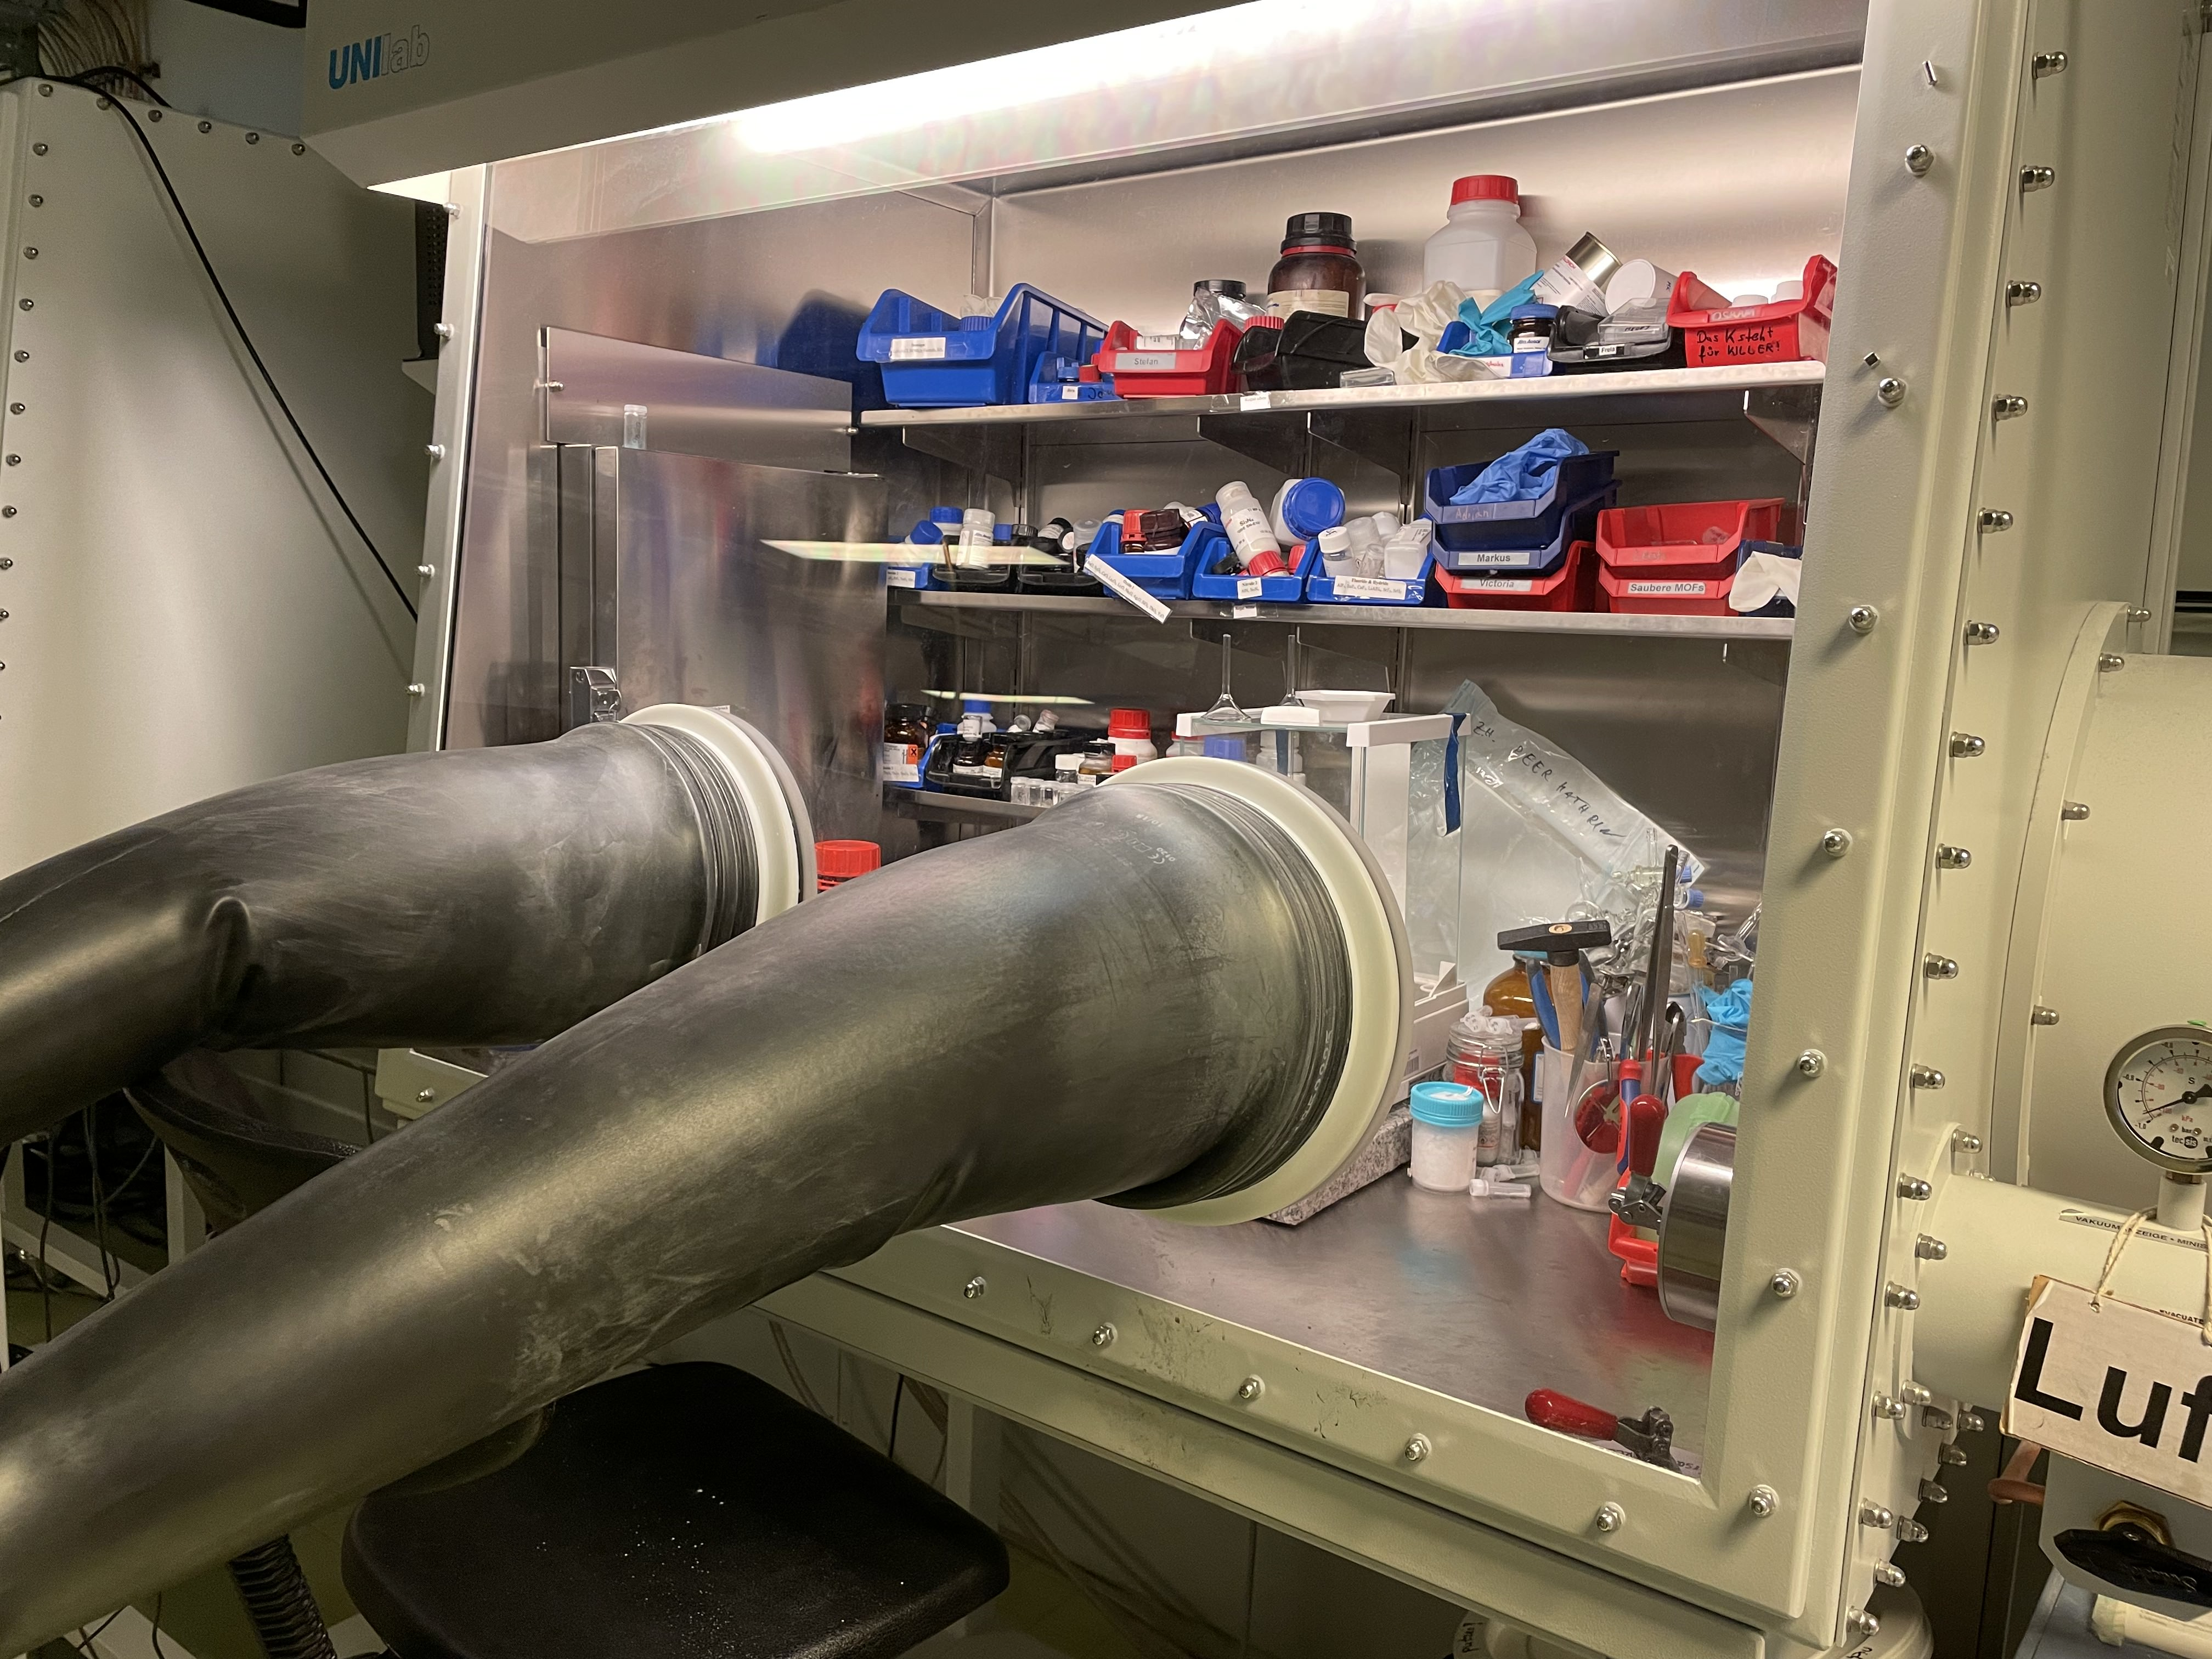
\includegraphics[height=8cm]{Images/Glovebox.jpg}
    \caption{MBraun Unilab (1200/780) Glovebox. Bildurheberin: Sabine Lerch, BSc.}
    \label{fig:glovebox}
\end{figure}

\subsection{Analytische Methoden}
\subsubsection{Röntgenpulverdiffraktometrie}
Alle im Praktikum durchgeführten Ansätze wurden mittels Röntgenpulverdiffraktometrie analysiert, wofür die fein gemörserte Probe entweder zwischen zwei Polyacetatfolien befestigt wird, oder in einer dünnen Kapillare eingeschlossen wird.
Die so präparierte Probe wird im Probenträger befestigt und dann ins STOE Stadi P Pulverdiffraktometer der Firma STOE \& Cie GmbH, dargestellt in Abbildung \ref{fig:stoe},  eingesetzt, wo mittels Mo-$K_{\alpha}$-Strahlung die Analyse erfolgt.~\cite{StoeP}
Die Detektion der Beugung erfolgt über einen Mythen 1K-Detektor (Dectris) und die so erhaltenen Diffraktogramme konnten an der WinXPOW Software qualitativ ausgewertet werden~\cite{Stoe}.

\begin{figure}[H]
    \centering
    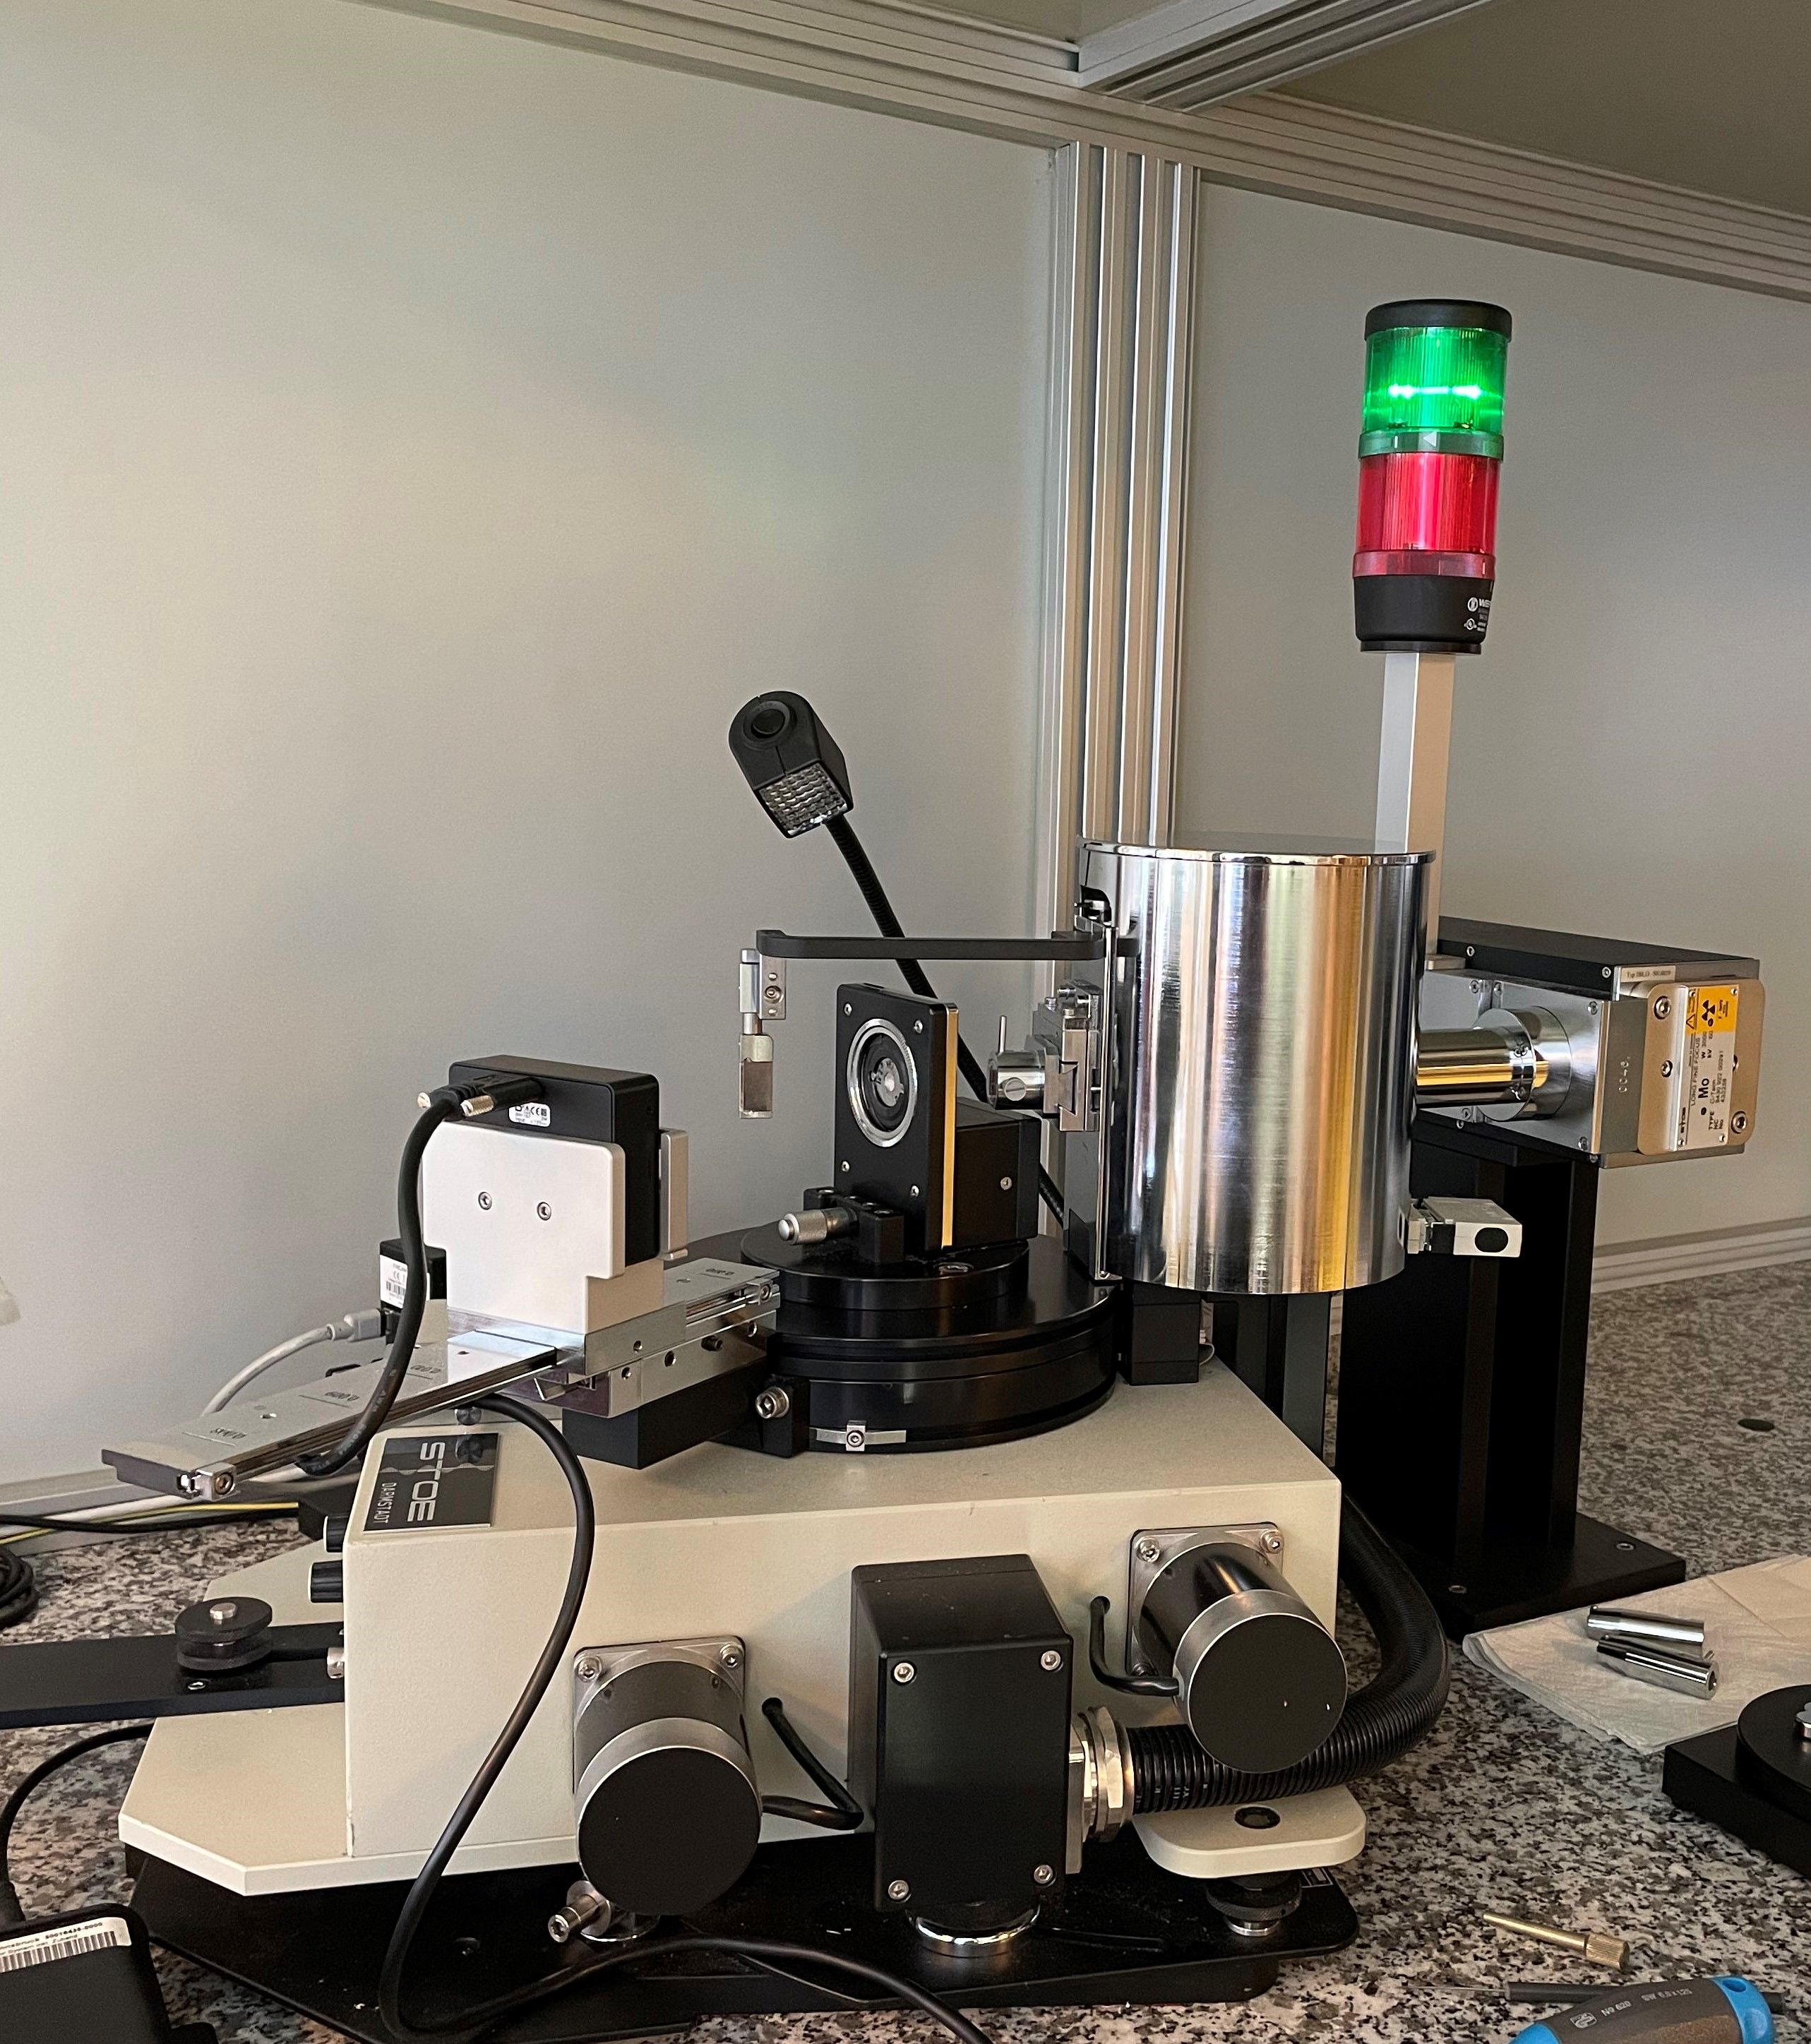
\includegraphics[height=8cm]{Images/Pulverdiff.jpg}
    \caption{Stoe Stadi P Pulverdiffraktometer. Bildurheberin: Sabine Lerch, BSc.}
    \label{fig:stoe}
\end{figure}

\subsubsection{Einkristallröntgendiffraktometrie}
Zu Übungszwecken wurden am Polarisationsmikroskop über Drehung des Polarisationsfilters Einkristalle isoliert.
Da zur Zeit des Praktikums jedoch technische Probleme am D8 Quest Einkristalldiffraktometers der Firma Bruker, dargestellt in Abbildung \ref{fig:brukeri}, auftraten, konnten die so präparierten Proben vorerst nicht weiter analysiert werden.

\begin{figure}[H]
    \centering
    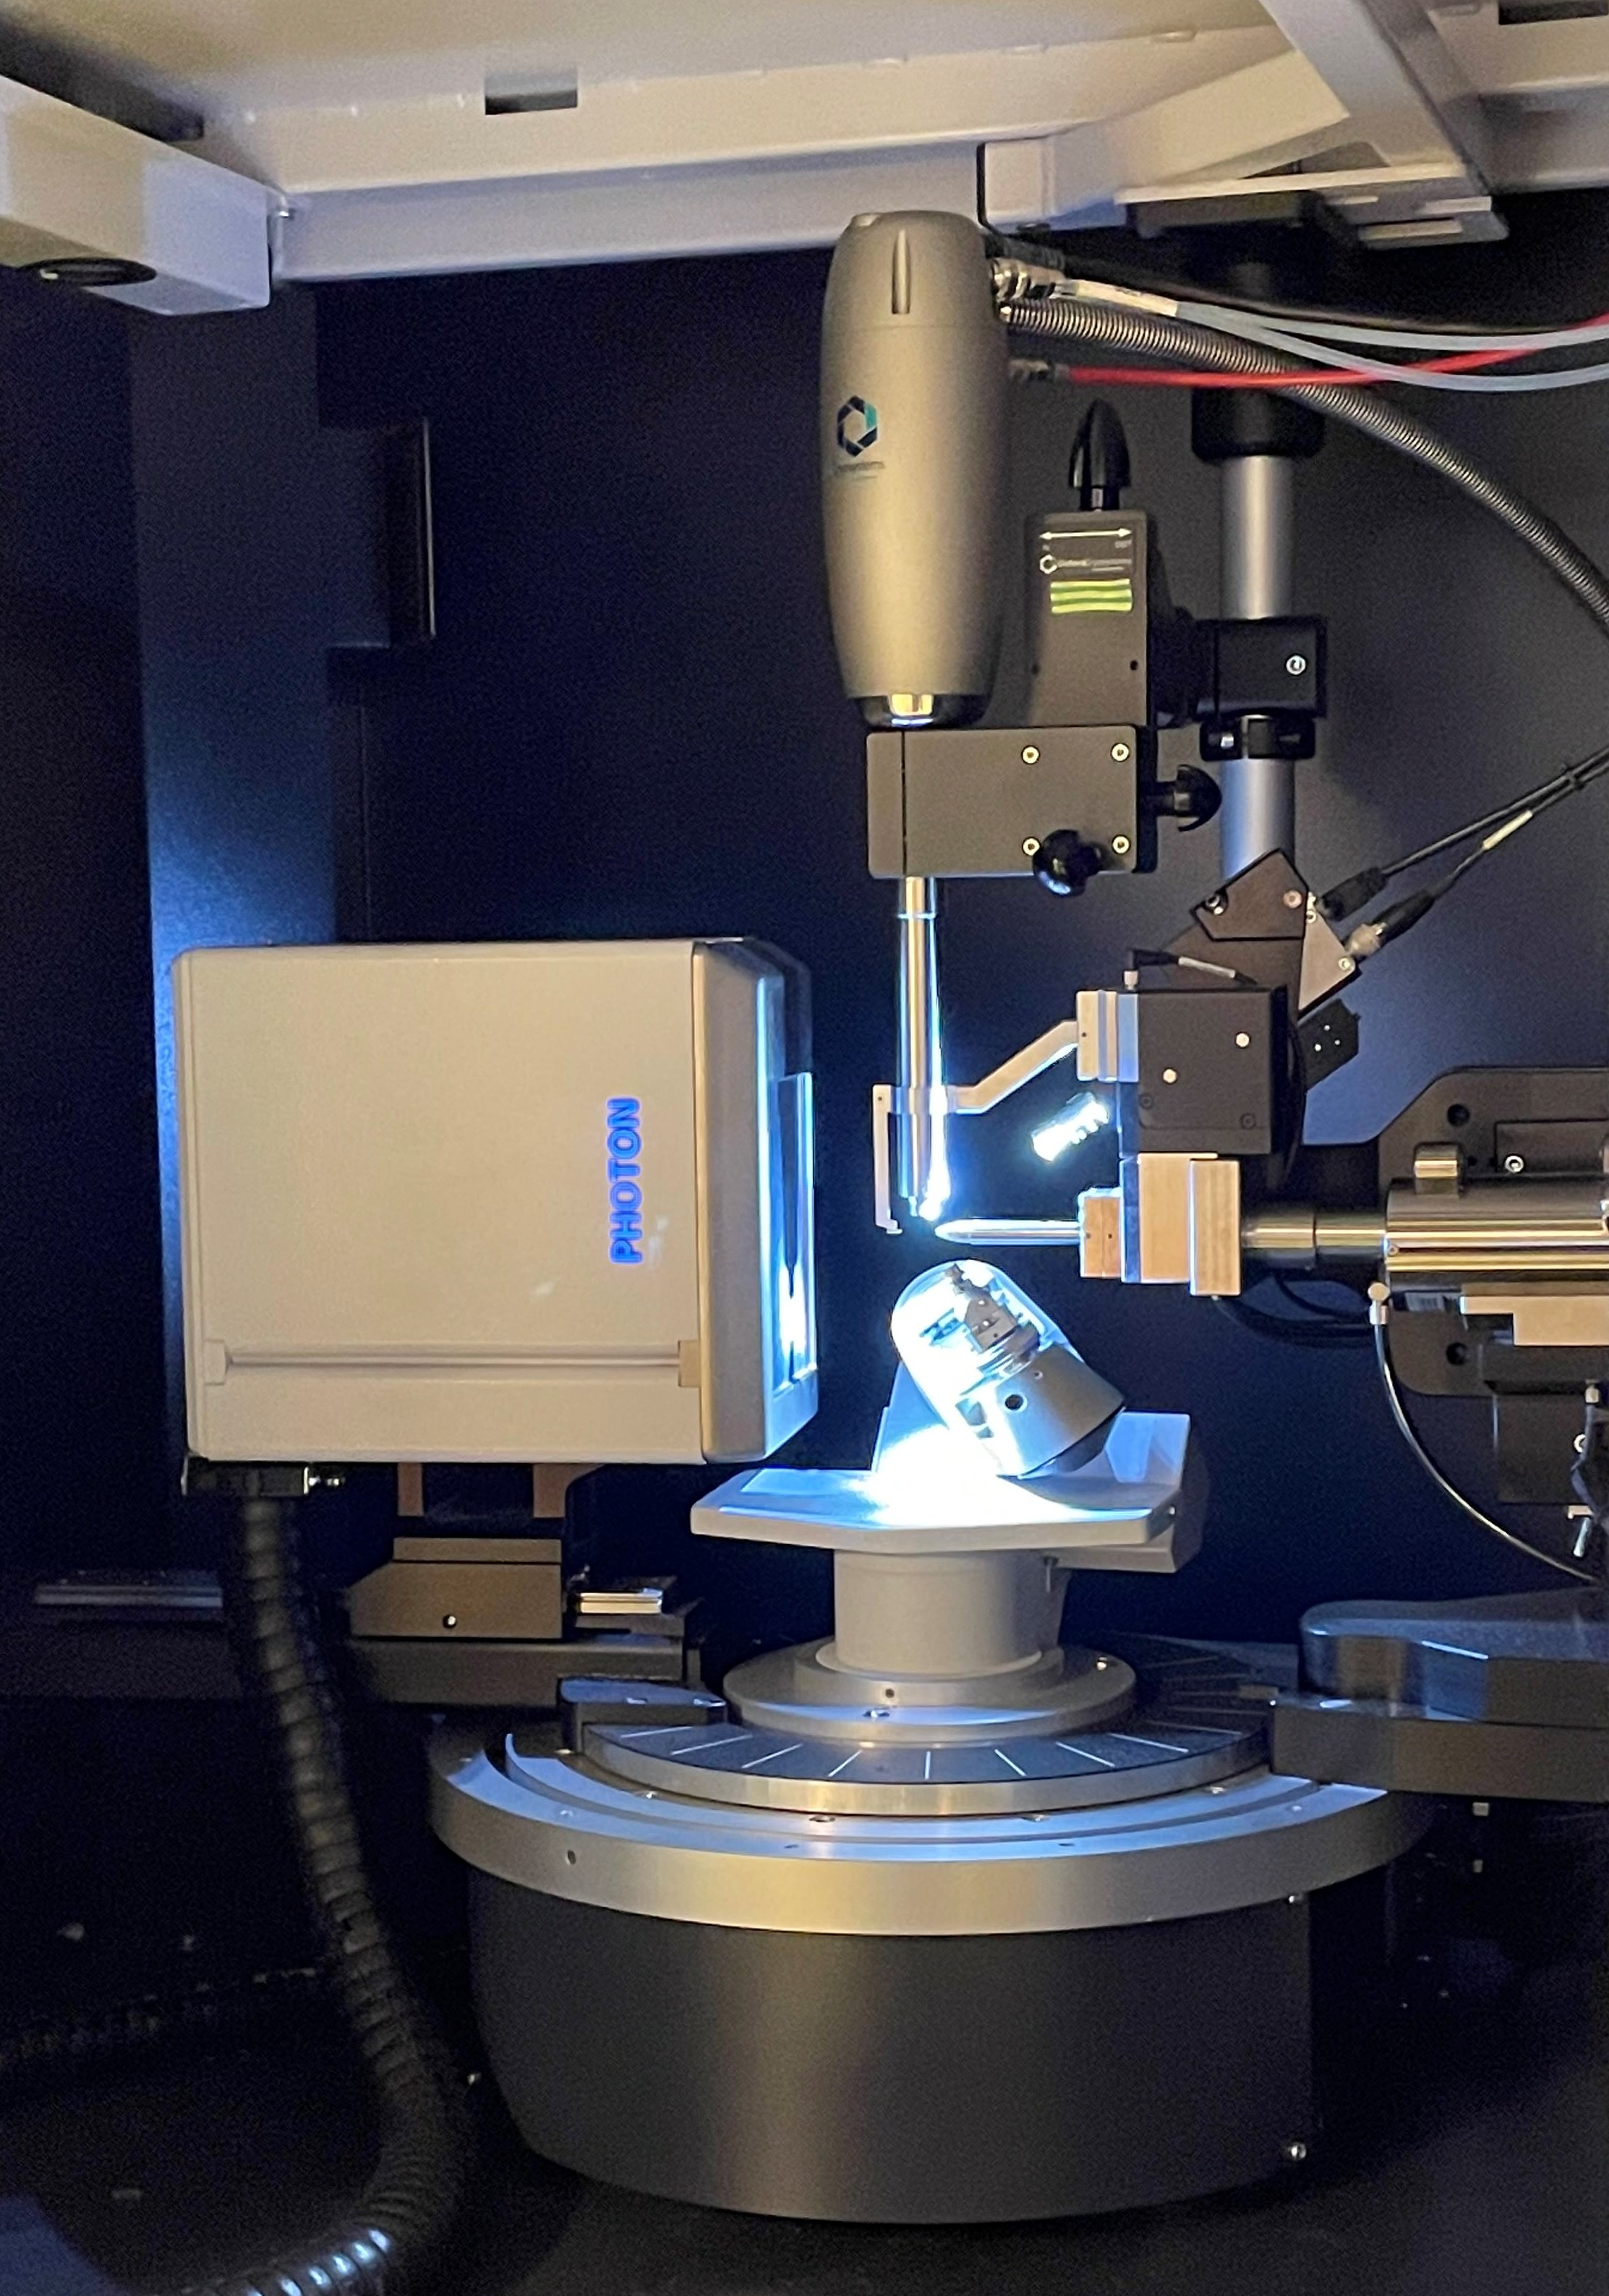
\includegraphics[height=8cm]{Images/Einkristalldiff.jpg}
    \caption{Zum Zeitpunkt des Praktikums nicht betriebsfähiges Bruker D8 Quest Einkristalldiffraktometer. Bildurheberin: Sabine Lerch, BSc.}
    \label{fig:brukeri}
\end{figure}

\subsubsection{Rasterelektronenmikroskopie}
Zur Einführung in die Rasterelektronenmikroskopie wurden verschiedene Proben im Clara Rasterelektronenmikroskop der Firma TESCAN untersucht.
Mittels dieser Methode können in kürzester Zeit hochauflösende Aufnahmen von Oberflächen bis in den Nanometer-bereich aufgenommen werden.
Hierbei werden Elektronen auf die Probe geschossen, wobei für die Feststoffanalyse vor allem zwei Arten der Detektion von Bedeutung sind:
Sekundärelektronen, welche aus der Probe herausgelöst wurden, erlauben eine hohe topographische Auflösung der Probe. 
Von der Probe rückgestreute Elektronen hingegen dienen zur chemischen Analyse der Probenmaterialien, da unterschiedliche Stoffe unterschiedliche Rückstrahlemissionen aufweisen und somit in unterschiedlichen Grauwerten dargestellt werden.

\begin{figure}[H]
    \centering
    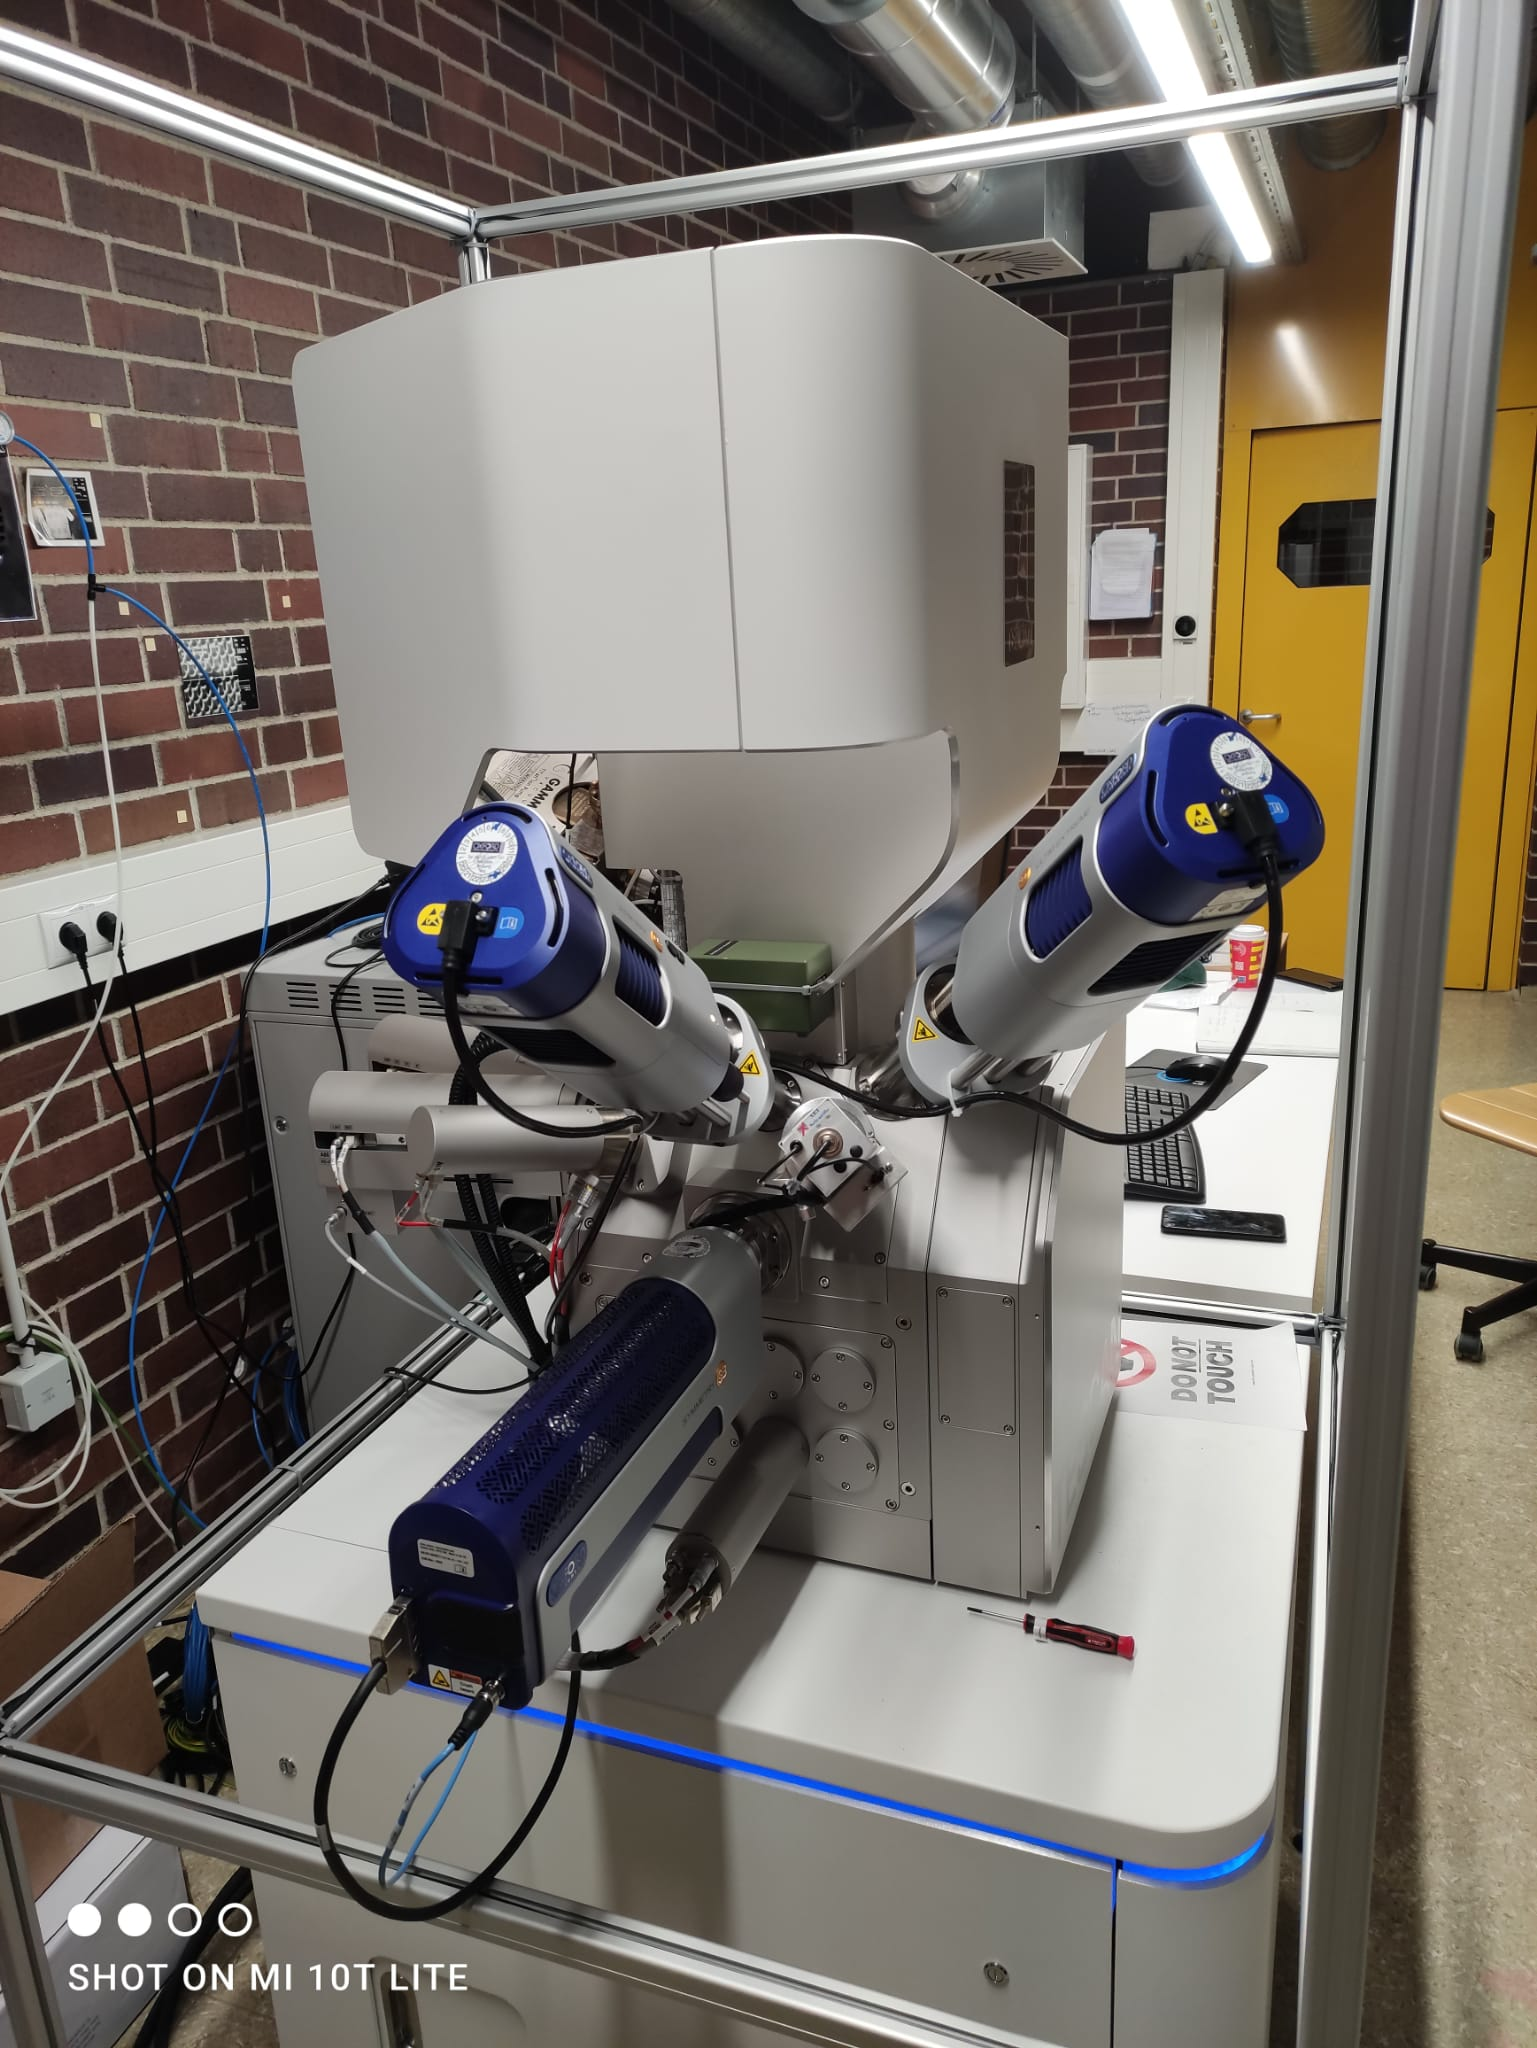
\includegraphics[height=8cm]{Images/REM.jpeg}
    \caption{TESCAN Clara Rasterelektronenmikroskop.}
\end{figure}

\begin{figure}[H]
    \centering
    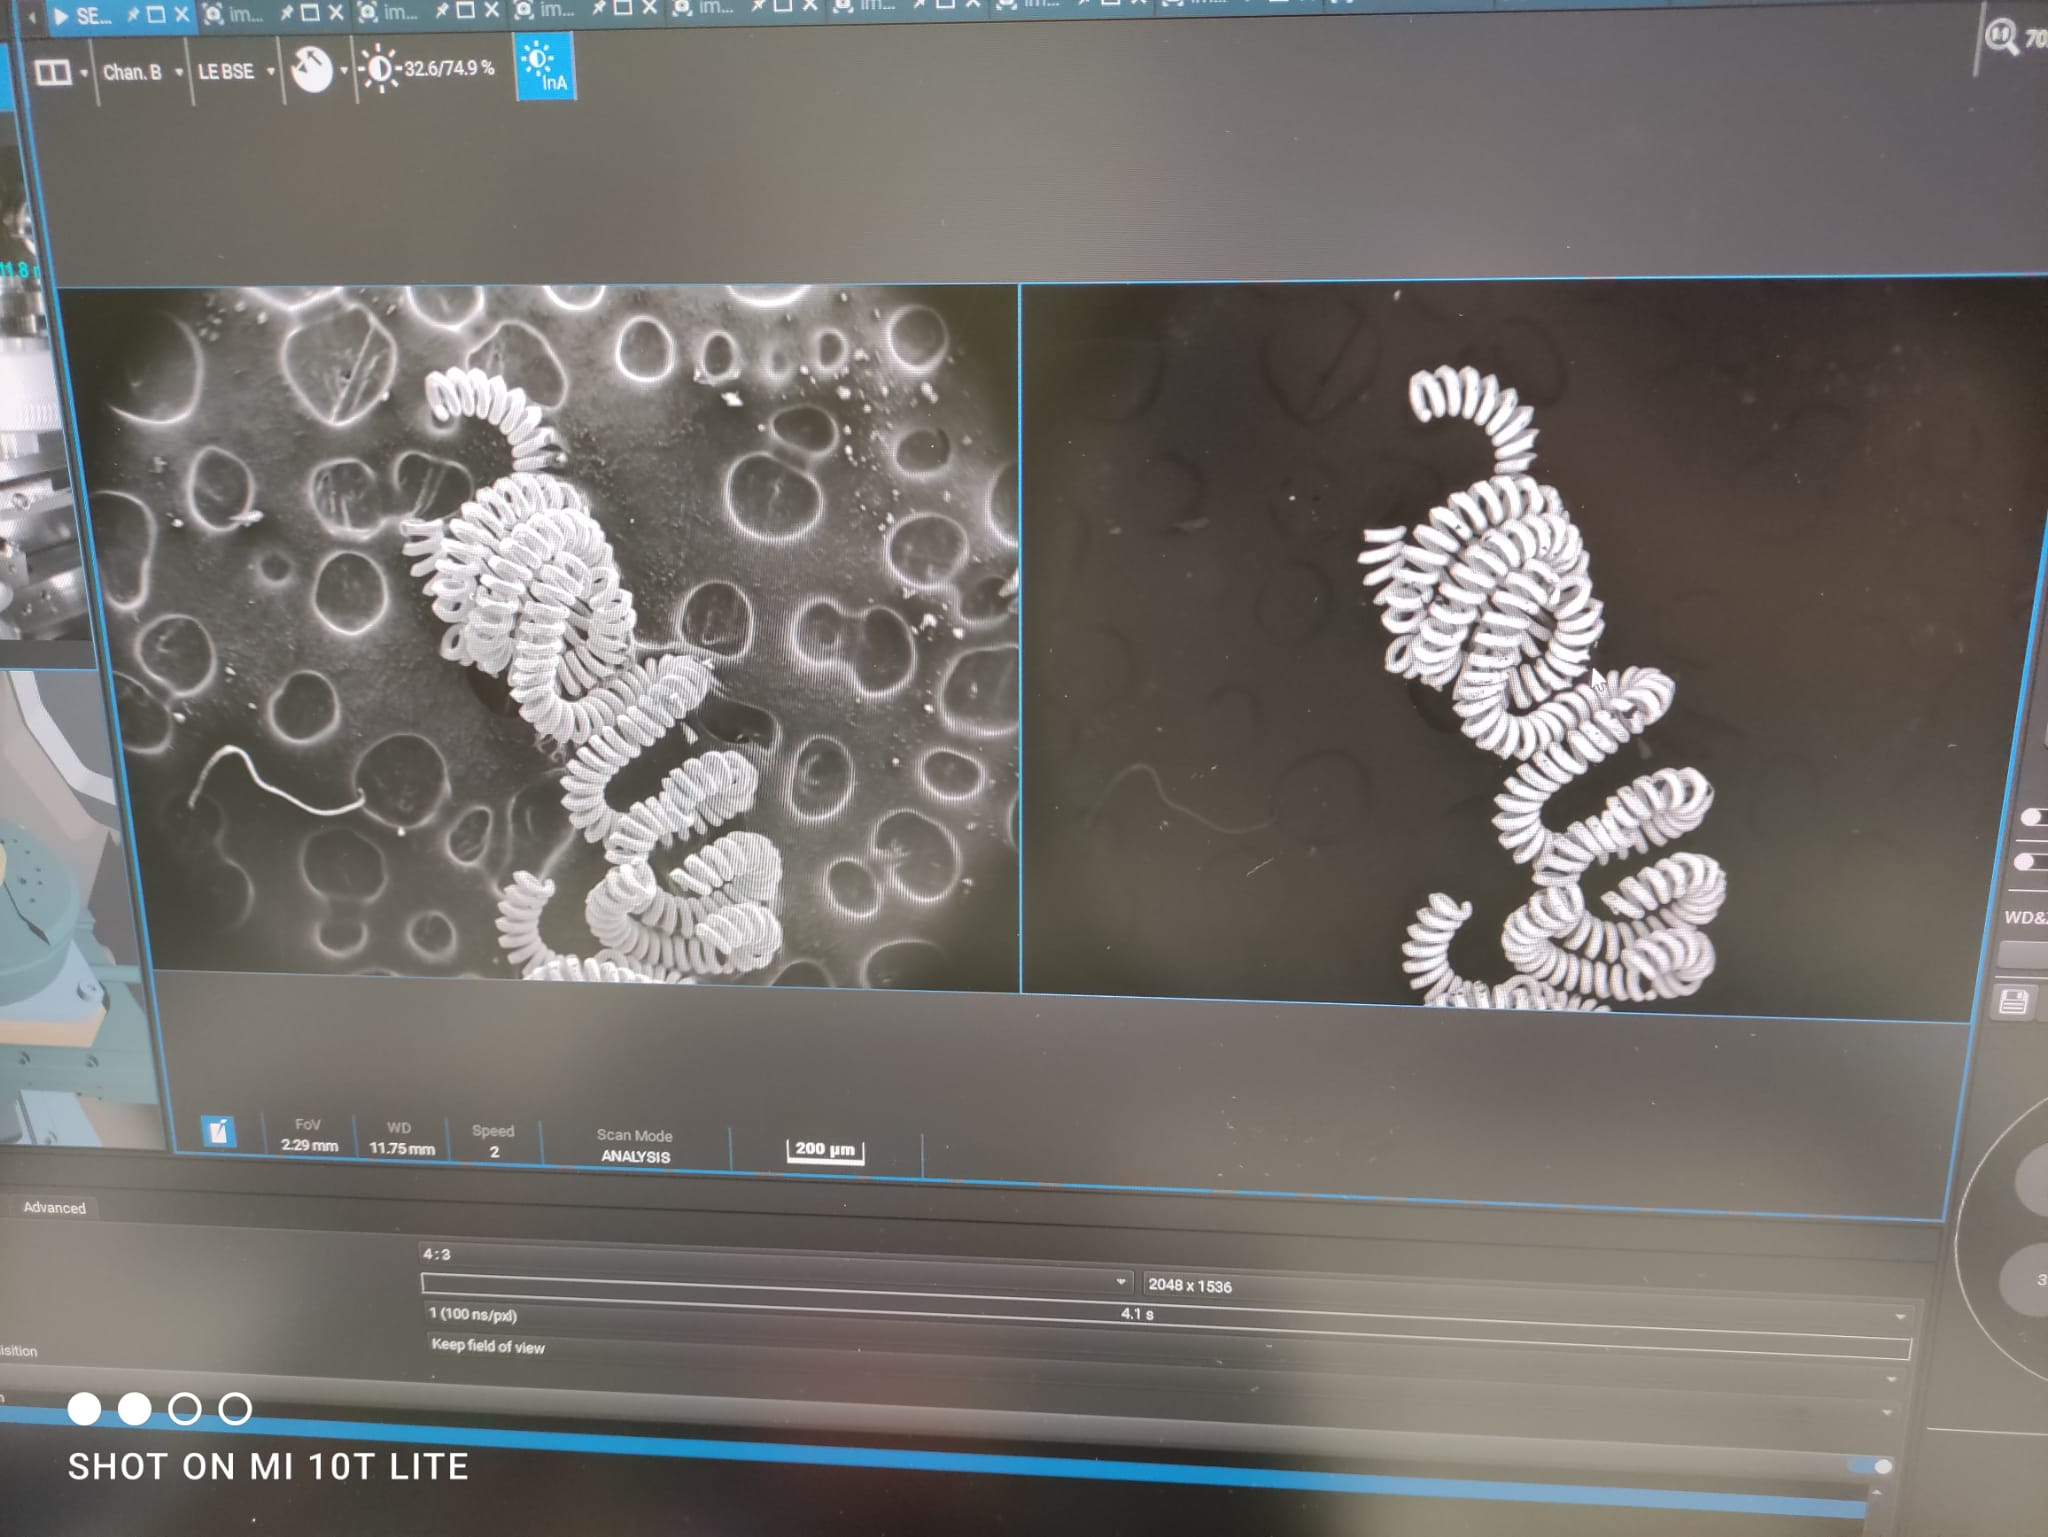
\includegraphics[height=8cm]{Images/REM1.jpeg}
    \caption{REM-Bild eines Wolframdrahtes über Sekundärelektronendetektion (links) und Rückstreuelektronendetektion (rechts).}
\end{figure}

\section{Hochdruckansätze}
\subsection{IW-165: \ce{GaB4O6N} : \ce{Ti^3+}}
\subsubsection{Experimentelle Durchführung}
Die in Tabelle~\ref{tab:1} aufgeführten Precursor wurden in einem 18/11 Assembly mit Goldkapsel in der Hochdruckpresse bei 6 GPa und 1000 \si{\degreeCelsius} wie im Pressenprogramm in Tabelle \ref{tab:2} aufgeführt behandelt.

\begin{table}[H]
    \centering
    \caption{Precursor Einwaage für den IW-165 Ansatz.}
    \begin{tabular}{|c|c|c|c|}
        \hline
        \textbf{Precursor} & \textbf{Masse} & \textbf{Stoffmenge} & \textbf{Äquivalente}  \\
        & \textbf{(mg)} & \textbf{(mmol)} &  \\
        \hline
        \ce{H3BO3} & 36.88 & 0.6 & 1\\
        \ce{Ga2O3} & 27.61 & 0.15 & 0.25 \\
        \ce{BN} & 14.49 & 0.58 & 0.97 \\
        \ce{Ti2O3} & 1.77 & 0.012 & 0.02 \\
        \hline
    \end{tabular}
    \label{tab:1}
\end{table}

\begin{table}[H]
    \centering
    \caption{Pressenprogramm für den IW-165 Ansatz.}
    \begin{tabular}{|c|c|c|c|c|}
        \hline
        \textbf{Öldruck} & \textbf{Probendruck} & \textbf{Heizleistung} & \textbf{Probentemperatur} & \textbf{Haltezeit}\\
        \textbf{(Bar)} & \textbf{(GPa)} & \textbf{(\%)} & \textbf{(\si{\degreeCelsius})} & \textbf{(min)} \\
        \hline
        179 & 6 & - & - &  200   \\
        179 & 6 & 48& 1000 &  10   \\
        179 & 6 & 48 & 1000 &  20   \\
        179 & 6 & 39 & 700 &  60   \\
        5 & - & - & - & 720   \\ 
        \hline
    \end{tabular}
    \label{tab:2}
\end{table}

\subsubsection{Auswertung}
Die Analyses des schwach violetten Produkts im Pulverdiffraktometer ist in Abbildung~\ref{fig:1} dargestellt.

\begin{figure}[H]
    \centering
    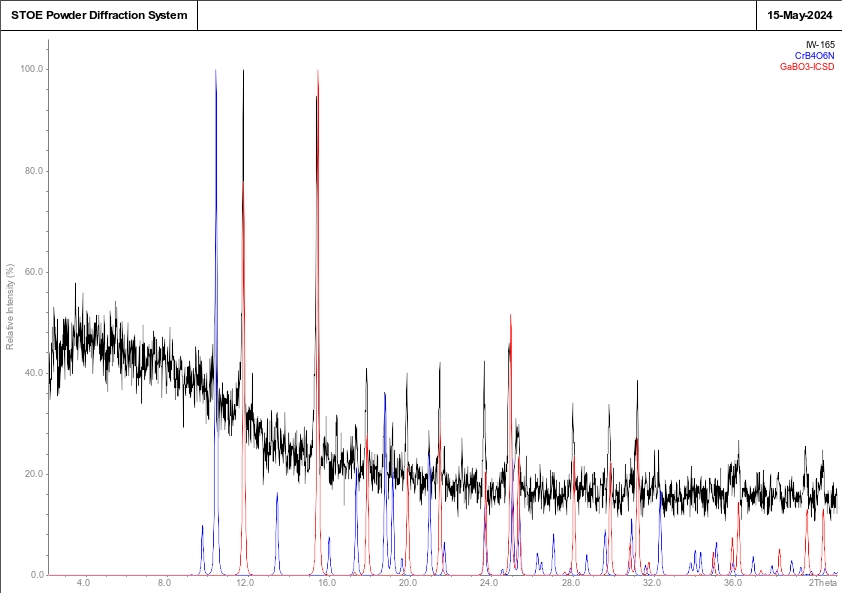
\includegraphics[height=8cm]{Images/165.jpg}
    \caption{Diffraktogramm des IW-165 Ansatzes mit theoretischen Pulverdiffraktogrammen von \ce{CrB4O6N} und \ce{GaBO3}.}
    \label{fig:1}
\end{figure}

\noindent Als Referenz dient die der Zielstruktur \ce{GaB4O6N} isotype \ce{CrB4O6N} Struktur (blau)~\cite{Fuchs2021}, wobei viele Reflexe im Diffraktogramm des IW-165 Produkts (schwarz) erkennbar sind.
Offensichtlich finden sich im Produkt auch \ce{GaBO3} Nebenprodukte (rot), wie zum Beispiel am intensiven Reflex bei 2$\theta$ = 15.5\si{\degree} zu erkennen ist.
Nichtsdestotrotz scheint das gewünschte Produkt vorhanden zu sein.

\noindent Zusätzlich zur Röntgenpulverdiffraktometrie wurde eine \textit{single grain laser luminescene (SGLL)} Messung der Probe durchgeführt, wobei die Lumineszenz der Probe bei Bestrahlung durch einen Laser gemessen wurde~\cite{Duller1999}.
Abbildung \ref{fig:SGLL} zeigt das so erhaltene Spektrum.

\begin{figure}[H]
    \centering
    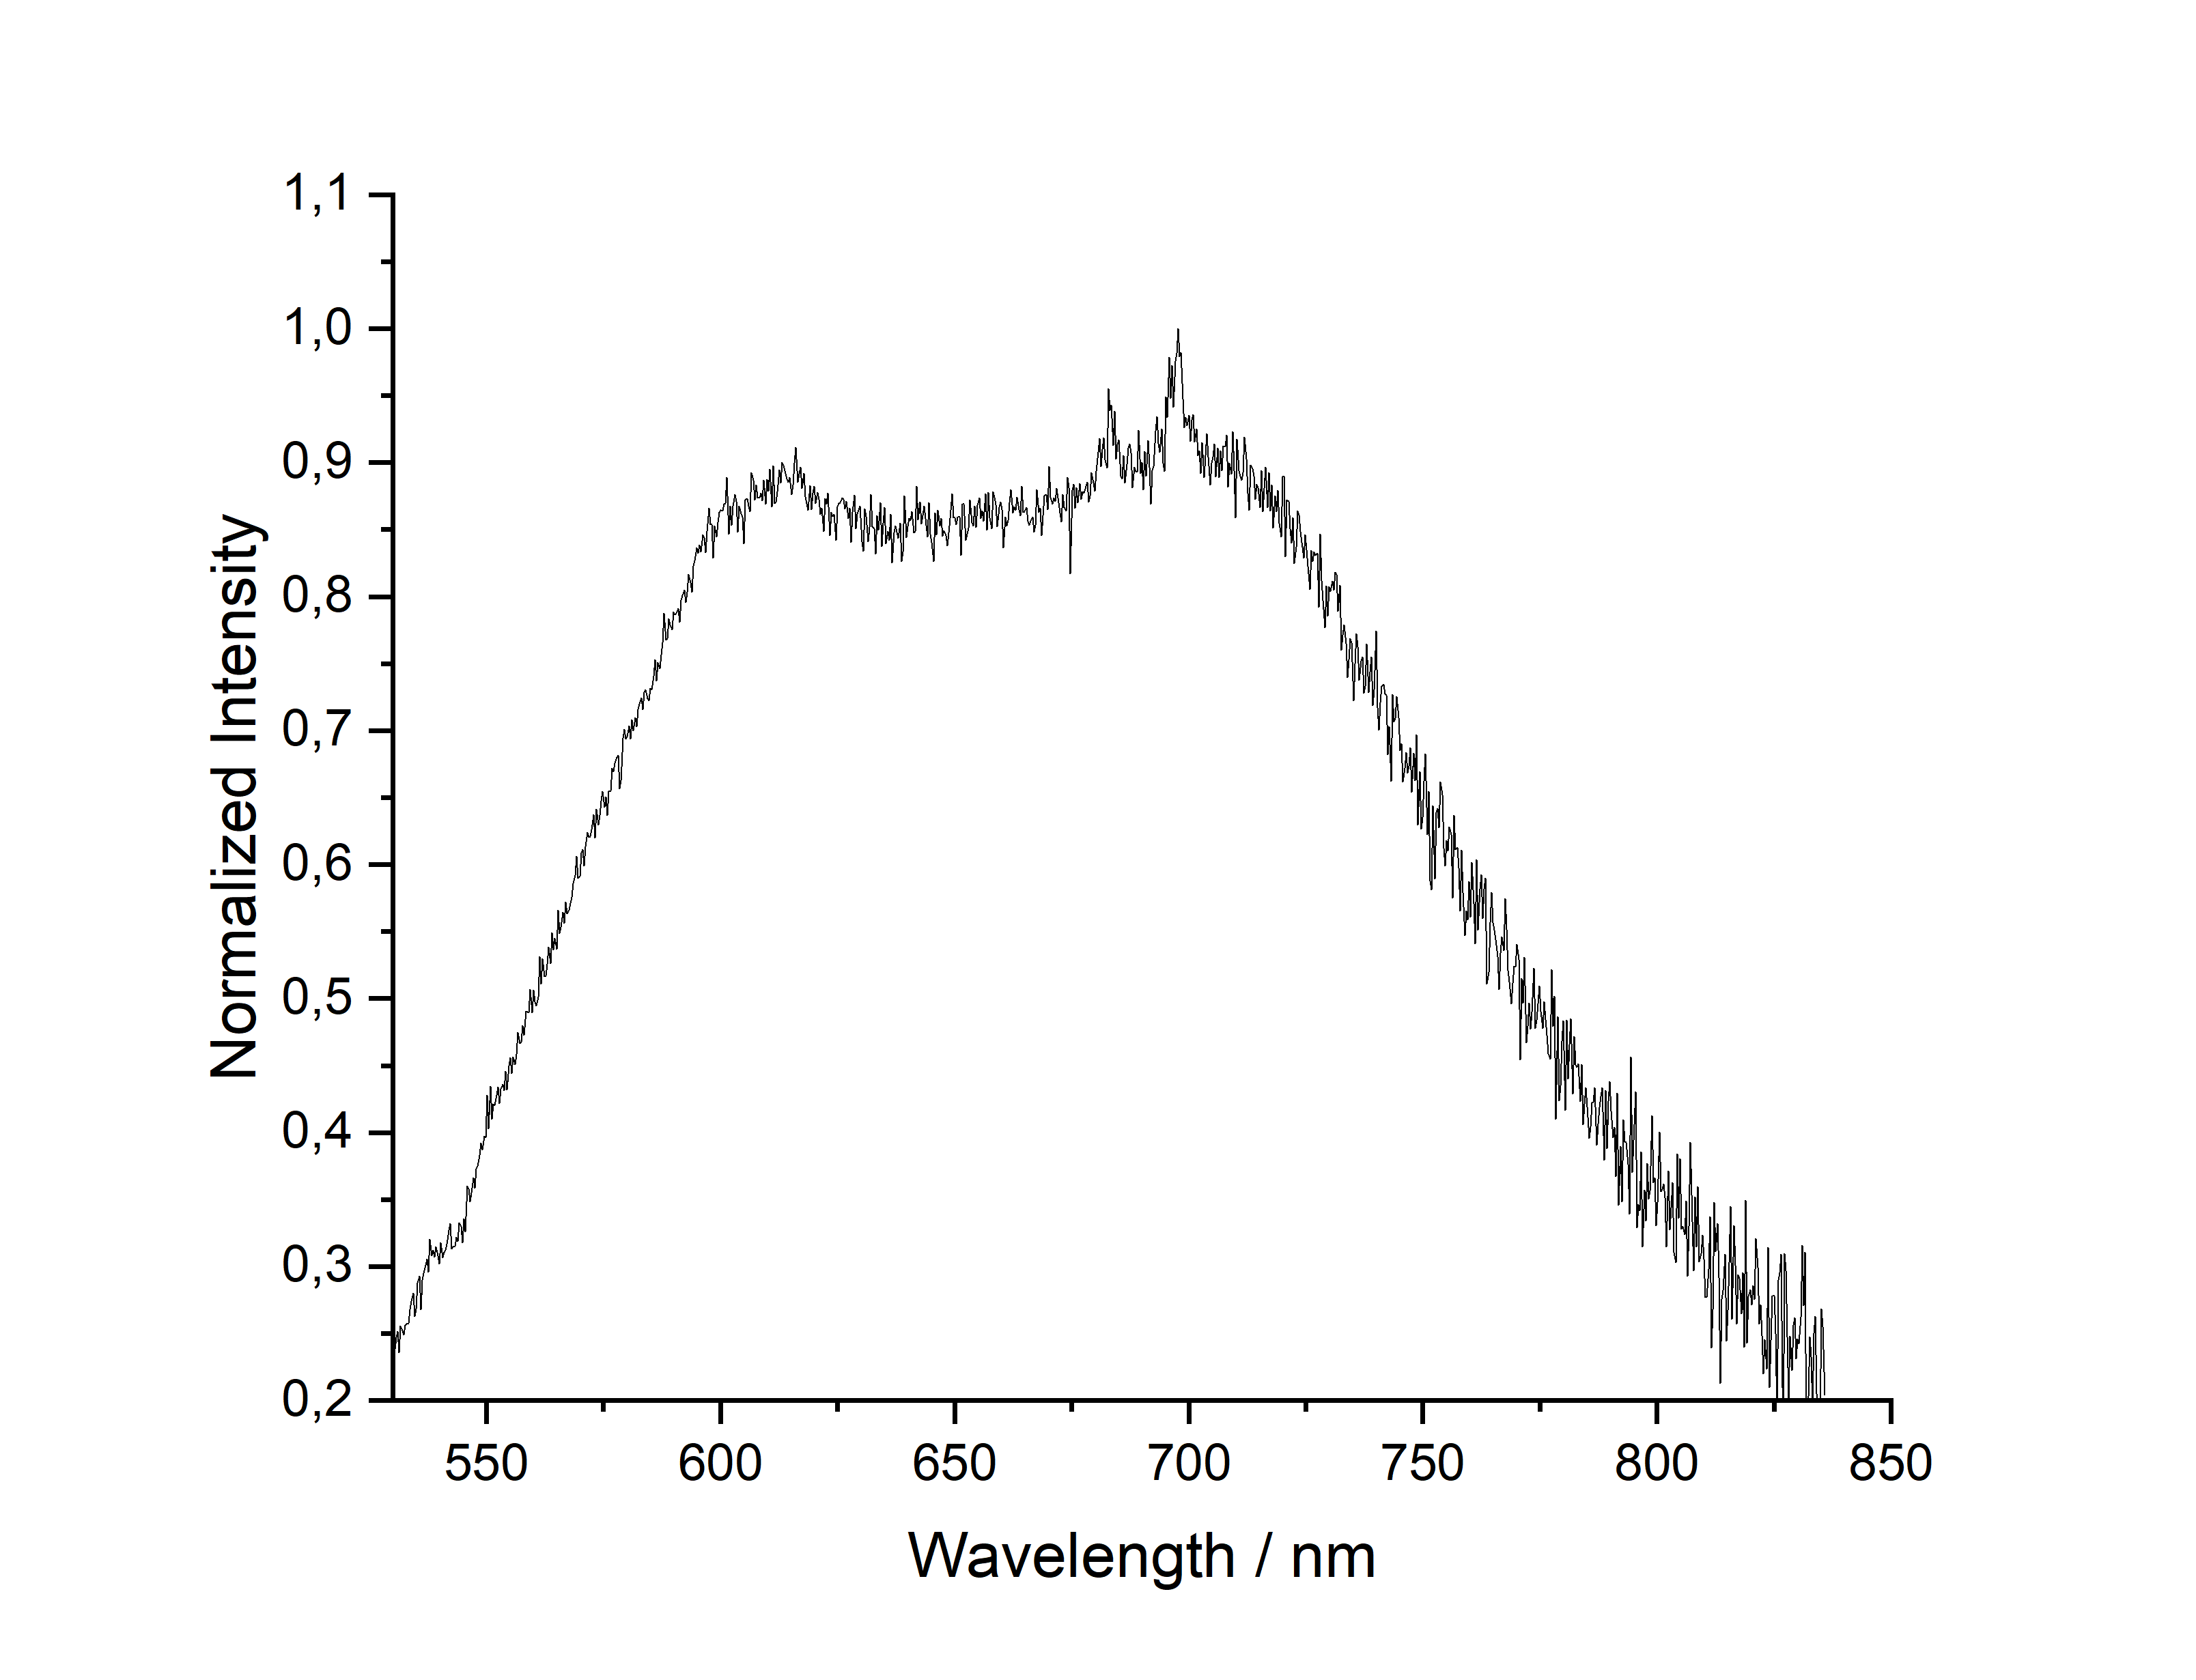
\includegraphics[height=8cm]{Images/IW_165_single_grain_4sec_avg6.png}
    \caption{SGLL Spektrum des IW-165 Ansatzes.}
    \label{fig:SGLL}
\end{figure}

\noindent Trotz markanter Lumineszenz-Peaks im Bereich zwischen 675 und 700 nm können diese nicht eindeutig dem \ce{GaB4O6N} Produkt zugeordnet werden, da wie bereits im Diffraktogramm ersichtlich \ce{GaBO3} Nebenprodukte vorhanden sind. 
Ein echtes single grain Verfahren, also die Behandlung eines Einzelkorns unter Vorraussetzung der mittels Einkristallröntgendiffraktometrie identifizierten Phase, könnte hierbei weitere Aufschlüsse geben.

\subsection{IW-166: \ce{GaB4O6N}}
\subsubsection{Experimentelle Durchführung}
Die in Tabelle~\ref{tab:3} aufgeführten Precursor wurden in einem 14/8 Assembly mit Platinkapsel in der Hochdruckpresse bei 9 GPa und 1200 \si{\degreeCelsius} wie im Pressenprogramm in Tabelle \ref{tab:4} aufgeführt behandelt.
Ziel war eine metastabile Hochdruckphase von \ce{GaB4O6N} mit möglichst wenig \ce{GaBO3} Nebenprodukten zu erhalten.

\begin{table}[H]
    \centering
    \caption{Precursor Einwaage für den IW-166 Ansatz.}
    \begin{tabular}{|c|c|c|c|}
        \hline
        \textbf{Precursor} & \textbf{Masse} & \textbf{Stoffmenge} & \textbf{Äquivalente}  \\
        & \textbf{(mg)} & \textbf{(mmol)} &  \\
        \hline
        \ce{H3BO3} & 39.62 & 0.65  & 1 \\
        \ce{Ga2O3} & 24.43 & 0.13 & 0.2 \\
        \ce{BN} & 15.94 & 0.64 & 0.98 \\
        \hline
    \end{tabular}
    \label{tab:3}
\end{table}

\begin{table}[H]
    \centering
    \caption{Pressenprogramm für den IW-166 Ansatz.}
        \begin{tabular}{|c|c|c|c|c|}
            \hline
            \textbf{Öldruck} & \textbf{Probendruck} & \textbf{Heizleistung} & \textbf{Probentemperatur} & \textbf{Haltezeit}\\
            \textbf{(Bar)} & \textbf{(GPa)} & \textbf{(\%)} & \textbf{(\si{\degreeCelsius})} & \textbf{(min)} \\
            \hline
            235 & 9 & - & - &  200   \\
            235 & 9 & 40& 1200 &  10   \\
            235 & 9 & 40 & 1200 &  20   \\
            235 & 9 & 32 & 900 &  60   \\
            5 & - & - & - & 580   \\ 
            \hline
    \end{tabular}
    \label{tab:4}
\end{table}

\subsubsection{Auswertung}
Aufgrund technischer Probleme am Pulverdiffraktometer konnte die Analyse des IW-166 Ansatzes nicht durchgeführt werden.

\subsection{IW-168: \ce{GaB4O6N} }
\subsubsection{Experimentelle Durchführung}
Die in Tabelle~\ref{tab:5} aufgeführten Precursor wurden in einem 14/8 Assembly mit Platinkapsel in der Hochdruckpresse bei 7 GPa und 1100 \si{\degreeCelsius} wie im Pressenprogramm in Tabelle \ref{tab:6} aufgeführt behandelt.
Ziel war erneut eine metastabile Hochdruckphase von \ce{GaB4O6N} mit möglichst wenig \ce{GaBO3} Nebenprodukten zu erhalten.

\begin{table}[H]
    \centering
    \caption{Precursor Einwaage für den IW-168 Ansatz.}
    \begin{tabular}{|c|c|c|c|}
        \hline
        \textbf{Precursor} & \textbf{Masse} & \textbf{Stoffmenge} & \textbf{Äquivalente}  \\
        & \textbf{(mg)} & \textbf{(mmol)} &  \\
        \hline
        \ce{H3BO3} & 39.73 & 0.64  & 1 \\
        \ce{Ga2O3} & 24.44 & 0.13 & 0.2 \\
        \ce{BN} & 15.87 & 0.64 & 1.00 \\
        \hline
    \end{tabular}
    \label{tab:5}
\end{table}

\begin{table}[H]
    \centering
    \caption{Pressenprogramm für den IW-168 Ansatz.}
    \begin{tabular}{|c|c|c|c|c|}
        \hline
        \textbf{Öldruck} & \textbf{Probendruck} & \textbf{Heizleistung} & \textbf{Probentemperatur} & \textbf{Haltezeit}\\
        \textbf{(Bar)} & \textbf{(GPa)} & \textbf{(\%)} & \textbf{(\si{\degreeCelsius})} & \textbf{(min)} \\
        \hline
        170 & 7 & - & - &  180   \\
        170 & 7 & 37& 1100 &  10   \\
        170 & 7 & 37 & 1100 &  10   \\
        5 & - & - & - & 720   \\ 
        \hline
    \end{tabular}
    \label{tab:6}
\end{table}

\subsubsection{Auswertung}
Die Analyses des farblosen Produkts im Pulverdiffraktometer ist in Abbildung~\ref{fig:2} dargestellt.

\begin{figure}[H]
    \centering
    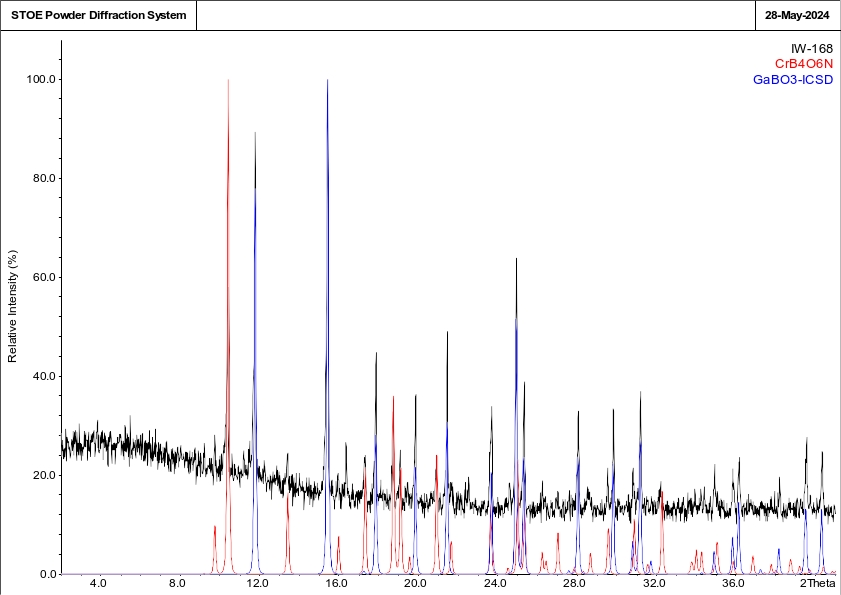
\includegraphics[height=8cm]{Images/168.jpg}
    \caption{Diffraktogramm des IW-168 Ansatzes mit Vergleichswerten.}
    \label{fig:2}
\end{figure}

\noindent Als Referenz dient erneut die der Zielstruktur \ce{GaB4O6N} (ICSD 181073) isotype \ce{CrB4O6N}
Struktur (rot). Obwohl offensichtlich das gewünschte Produkt entstanden ist, finden sich weiterhin viele Reflexe von GaBO3 Nebenprodukten (blau) im Diffraktogramm.

\subsection{STS-29: \ce{CuSb3Se5}}
\subsubsection{Experimentelle Durchführung}
Ziel dieses Versuchs war die Synthese einer metastablilen \ce{CuSb3Se5} Hochdruckphase bei einem Druck von 6 GPa, welche in einem vorherigen Ansatz (STS-13) bereits erfolgreich bei 9 GPa hergestellt wurde.
Die in Tabelle~\ref{tab:9} aufgeführten Precursorelemente wurden dazu unter Argonatmosphäre in einer Quarzampulle versiegelt und im Muffelofen eine Stunde bei 950 \si{\degreeCelsius} ausgeheizt und für 15 weiter Stunden gehalten, wonach die Ampulle im Wasserbad gequencht wurde.
Die abgekühlte Probe wurde daraufhin in einem 18/11 Assembly, ohne Platinkapsel und im \ce{BN}-Tiegel, in der Hochdruckpresse bei 6 GPa und 1000 \si{\degreeCelsius} wie im Pressenprogramm in Tabelle \ref{tab:10} aufgeführt behandelt.


\begin{table}[H]
    \centering
    \caption{Precursor Einwaage für den STS-29 Ansatz.}
    \begin{tabular}{|c|c|c|c|}
        \hline
        \textbf{Precursor} & \textbf{Masse} & \textbf{Stoffmenge} & \textbf{Äquivalente}  \\
        & \textbf{(mg)} & \textbf{(mmol)} & \\
        \hline
        \ce{Cu} & 23.15 & 0.35  & 1 \\
        \ce{Sb} & 133.05 & 1.09 & 3.08 \\
        \ce{Se} & 143.88 & 1.82 & 5.14 \\
        \hline
    \end{tabular}
    \label{tab:9}
\end{table}

\begin{table}[H]
    \centering
    \caption{Pressenprogramm für den STS-29 Ansatz.}
    \begin{tabular}{|c|c|c|c|c|}
        \hline
        \textbf{Öldruck} & \textbf{Probendruck} & \textbf{Heizleistung} & \textbf{Probentemperatur} & \textbf{Haltezeit}\\
        \textbf{(Bar)} & \textbf{(GPa)} & \textbf{(\%)} & \textbf{(\si{\degreeCelsius})} & \textbf{(min)} \\
        \hline
        180 & 6 & - & - &  150   \\
        180 & 6 & 48& 1000 &  10   \\
        180 & 6 & 48 & 1000 &  20   \\
        180 & 6 & 5 & - &  320   \\
        5 & - & - & - & 450   \\ 
        \hline
    \end{tabular}
    \label{tab:10}
\end{table}

\subsubsection{Auswertung}
Nach Extraktion des Produkts und Zerkleinerung im Mörser wurde ein Pulverdiffraktogramm in der Kapillare aufgenommen wurde, welches in Abbildung~\ref{fig:8} dargestellt ist.

\begin{figure}[H]
    \centering
    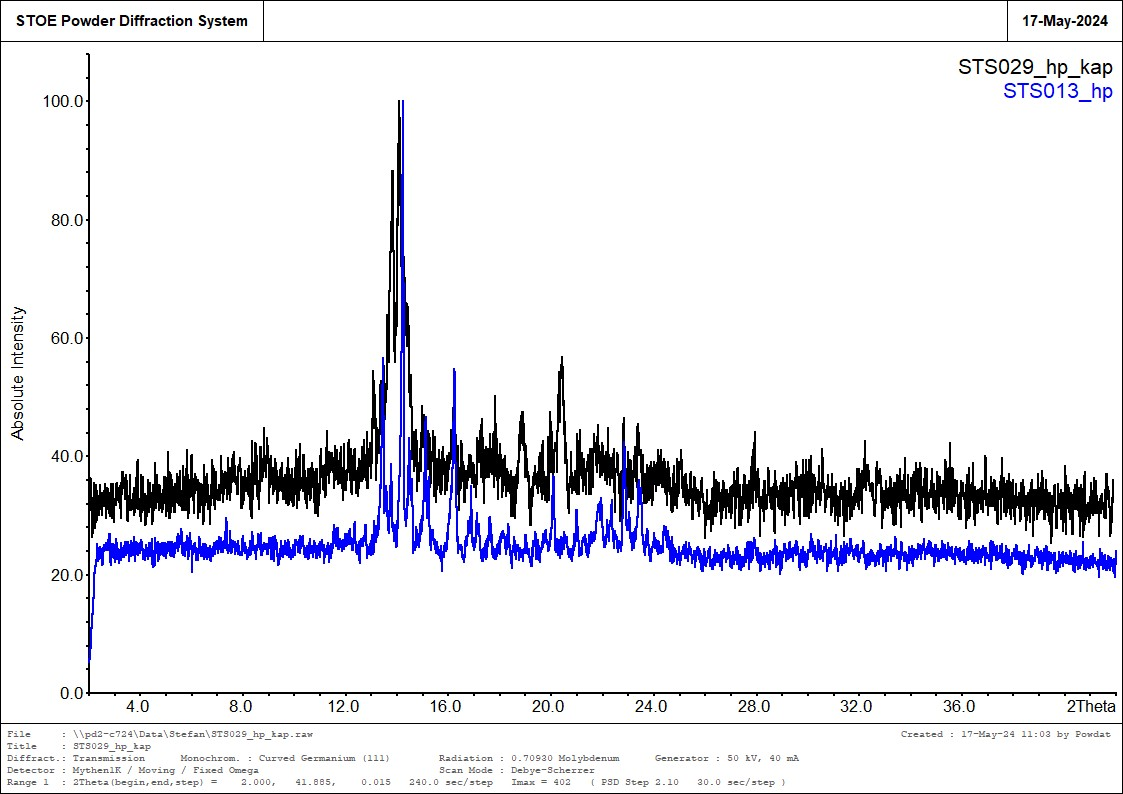
\includegraphics[height=8cm]{Images/STS029_hp.jpg}
    \caption{Diffraktogramm des STS-29 Ansatzes mit STS-13 als Referenz.}
    \label{fig:8}
\end{figure}

\noindent Die im Diffraktogramm des STS-29 Ansatzes (schwarz) erkennbaren Reflexe stimmen in großen Teilen gut mit denen des STS-13 Ansatzes (blaut) überein, wobei die zuätzlichen Reflexe auf das Vorhandensein von Nebenprodukten bzw. unerwünschten Phasen schließen lässt. 
Auch sind die Linien im Spektrum des STS-29 Ansatzes breiter und weniger scharf als die des STS-13 Ansatzes, was auf eine geringere Kristallinität des Produkts hindeutet.
Nichtsdestotrotz scheint die gewünschte Hochdruckphase jedoch auch bei einem Druck von 6 GPa zumindest in Teilen synthetisierbar zu sein, der höhere Drück von 9 GPa führt aber zu höherer Kristallinität.

\subsection{STS-92: \ce{Li_{1.33}MoS2}}
\subsubsection{Experimentelle Durchführung}

Im Rahmen der Forschung im Bereich der Festkörperbatterien wurde der Ansatz STS-92 zur Synthese von \ce{Li_{1.33}MoS2} durchgeführt, wobei eine Interkalation von Lithium in die Schichtstruktur von \ce{MoS2} stattfinden sollte.
Die in Tabelle~\ref{tab:11} aufgeführten Precursorelemente wurden in einem 18/11 Assembly in der Hochdruckpresse bei 8 GPa und 1000 \si{\degreeCelsius} wie im Pressenprogramm in Tabelle \ref{tab:12} aufgeführt behandelt. Die erwartete Reaktionsgleichung für die Synthese ist in Gleichung~\ref{eq:1} dargestellt.

\begin{table}[H]
    \centering
    \caption{Precursor Einwaage für den STS-92 Ansatz.}
    \begin{tabular}{|c|c|c|c|}
        \hline
        \textbf{Precursor} & \textbf{Masse} & \textbf{Stoffmenge} & \textbf{Äquivalente}  \\
        & \textbf{(mg)} & \textbf{(mmol)} & \\
        \hline
        \ce{Li2S} & 54.24 & 1.18  & 1 \\
        \ce{Mo} & 170.04 & 1.78 & 1.51 \\
        \ce{S} & 75.76 & 2.36 & 2.00 \\
        \hline
    \end{tabular}
    \label{tab:11}
\end{table}

\begin{table}[H]
    \centering
    \caption{Pressenprogramm für den STS-92 Ansatz.}
    \begin{tabular}{|c|c|c|c|c|}
        \hline
        \textbf{Öldruck} & \textbf{Probendruck} & \textbf{Heizleistung} & \textbf{Probentemperatur} & \textbf{Haltezeit}\\
        \textbf{(Bar)} & \textbf{(GPa)} & \textbf{(\%)} & \textbf{(\si{\degreeCelsius})} & \textbf{(min)} \\
        \hline
        245 & 8 & - & - &  205   \\
        245 & 8 & 48& 1000 &  10   \\
        245 & 8 & 48 & 1000 &  10   \\
        245 & 8 & 1 & - &  300   \\
        - & - & - & - & 615   \\ 
        \hline
    \end{tabular}
    \label{tab:12}
\end{table}

\begin{equation}
    \ce{2Li2S + 3Mo + 4S -> 3Li_{1.33}MoS2}
    \label{eq:1}
\end{equation}

\subsubsection{Auswertung}
Die Extraktion des Produkts und Zerkleinerung im Mörser erfolgte in der Glovebox unter Argonatmosphäre bevor das erhaltene Pulver im Pulverdiffraktometer in einer Kapillare analysiert wurde.
Das Diffraktogramm des Ansatzes STS-92 ist in Abbildung~\ref{fig:9} dargestellt.


\begin{figure}[H]
    \centering
    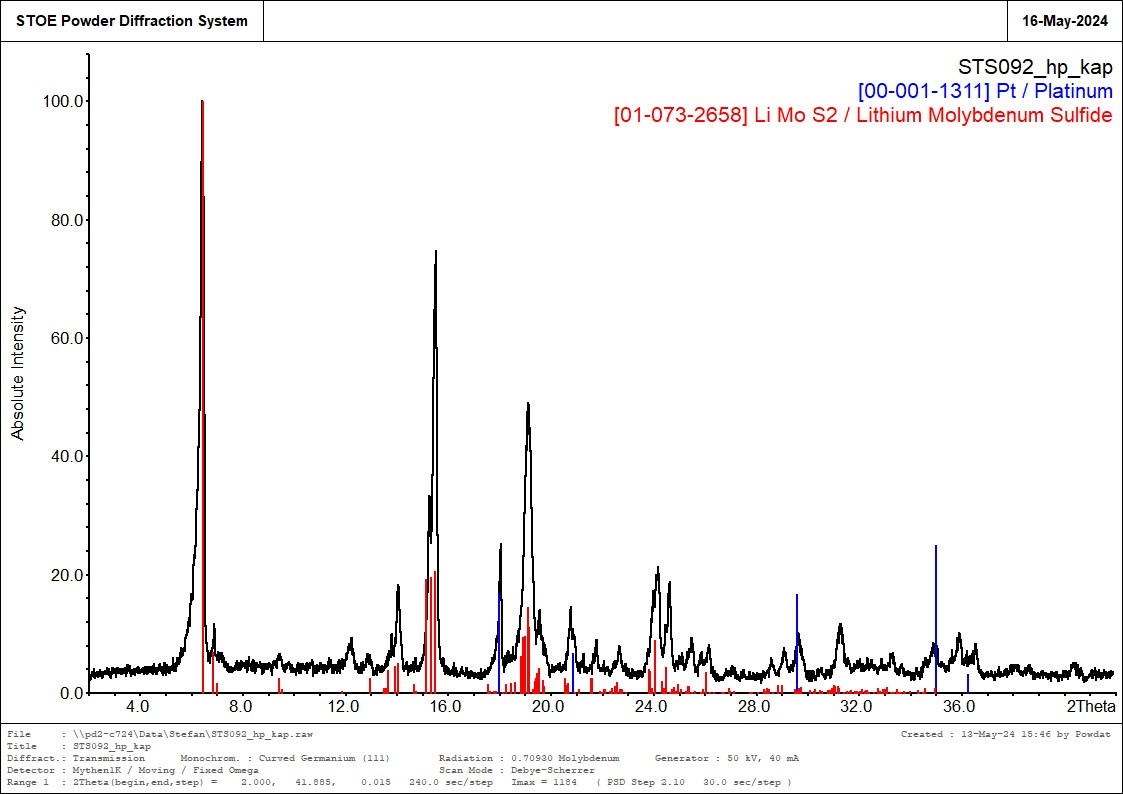
\includegraphics[height=8cm]{Images/STS_092.jpg}
    \caption{Diffraktogramm des STS-92 Ansatzes mit Vergleichswerten.}
    \label{fig:9}
\end{figure}

\noindent Aus den Überlappungen des hochauflösenden Diffraktogramms des STS-92 Ansatzes (schwarz) mit den Referenzwerten von \ce{LiMoS2} (rot) lässt sich schließen, dass das gesuchte Produkt in großen Teilen synthetisiert wurde und die gewünschte Interkalation von Lithium in die Schichtstruktur von \ce{MoS2} erfolgt ist.
Nichtsdestotrotz sind auch Verunreinigungen erkennbar, die laut Referenzwerten (blau) wohl auf die Platinkapsel zurückzuführen sind.

\section{Hochtemperaturansatz}
\subsection{STS-93: \ce{CuSb3Se5}}
\subsubsection{Experimentelle Durchführung}
In diesem Ansatz wurde die im vorherigen Ansatz STS-29 dem Hochdruckprogramm unterzogene Vorstufe erneut hergestellt.
Die in Tabelle~\ref{tab:13} aufgeführten Precursorelemente wurden unter Argonatmosphäre in einer Quarzampulle versiegelt und im Muffelofen eine Stunde bei 990 \si{\degreeCelsius} ausgeheizt und für 2 weitere Stunden gehalten, wonach die Ampulle im Wasserbad gequencht wurde.

\begin{table}[H]
    \centering
    \caption{Precursor Einwaage für den STS-93 Hochtemperaturansatz.}
    \begin{tabular}{|c|c|c|c|}
        \hline
        \textbf{Precursor} & \textbf{Masse} & \textbf{Stoffmenge} & \textbf{Äquivalente}  \\
        & \textbf{(mg)} & \textbf{(mmol)} & \\
        \hline
        \ce{Cu} & 38.63 & 0.60  & 1 \\
        \ce{Sb} & 221.87 & 1.82 & 3.03 \\
        \ce{Se} & 239.59 & 3.03 & 5.06 \\
        \hline
    \end{tabular}
    \label{tab:13}
\end{table}

\subsubsection{Auswertung}
Nach Zerkleinerung im Mörser wurde ein Pulverdiffraktogramm in der Kapillare aufgenommen wurde, welches in Abbildung~\ref{fig:10} dargestellt ist.

\begin{figure}[H]
    \centering
    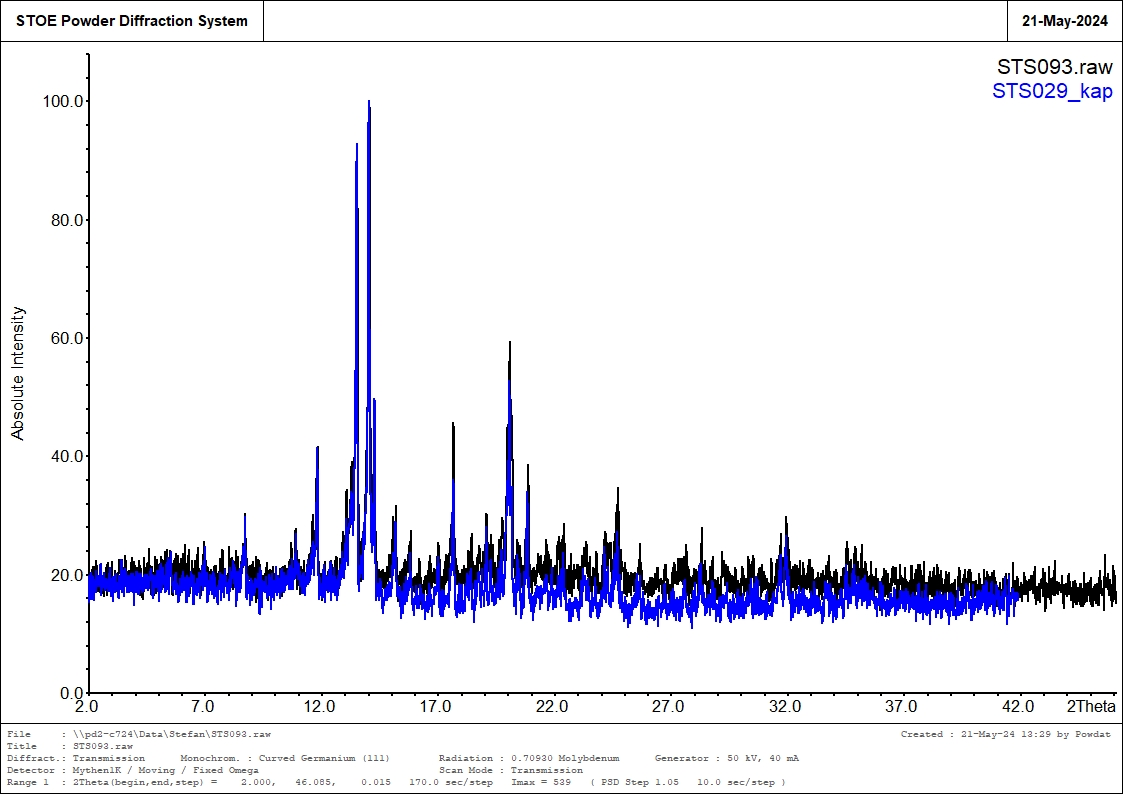
\includegraphics[height=8cm]{Images/STS093029_Fill.jpg}
    \caption{Diffraktogramm des STS-93 Hochtemperaturansatzes mit STS-29-Precursor als Referenz.}
    \label{fig:10}
\end{figure}

\noindent Aus den fast identischen Reflexen des STS-93 Ansatzes (schwarz) und des STS-29 Ansatzes (blau) lässt sich schließen, dass die gewünschte Vorstufe erwartungsgemäß synthetisiert wurde.

\section{Hydrothermalansätze}
\subsection{Experimentelle Durchführung}

Für die Hydrothermalansätze wurden fünf verschiedene Precursor-Gemenge in unterschiedlicher Zusammensetzungen unter wässrigen Bedingungen in Autoklaven gegeben und bei verschiedenen Temperaturen im Konvektionsofen behandelt.
Tabelle~\ref{tab:7} zeigt die Precursor und Mengen für die Ansätze A bis E.

\begin{table}[H]
    \centering
    \caption{Precursor Einwaage für die Hydrothermalansätze A bis E.}
    \begin{tabular}{|c|c|c|c|c|c|}
        \hline
        \textbf{Ansatz} & \textbf{Precursor} & \textbf{Masse} & \textbf{Stoffmenge} & \textbf{Äquivalente}  \\
        & & \textbf{(mg)} & \textbf{(mmol)} &  \\
        \hline
        A & \ce{Al(NO3)3*9H2O} & 243.10 & 0.648 & 1 \\
        & \ce{H3BO3} & 154.20 & 2.493 & 3.85 \\
        & \ce{NH4F} & 1.19 & 0.032 & 0.05 \\
        \hline
        B & \ce{Al(NO3)3*9H2O} & 380.56 & 1.014 & 1 \\
        & \ce{H3BO3} & 16.79 & 0.272 & 0.27 \\
        & \ce{NH4F} & 0.63 & 0.017 & 0.02 \\
        \hline
        C & \ce{Ga(NO3)3*8H2O} & 246.51 & 0.616 & 1 \\
        & \ce{H3BO3} & 152.96 & 2.474 & 4.02 \\
        & \ce{NH4F} & 1.80 & 0.049 & 0.08 \\
        \hline
        D & \ce{Ga2O3} & 81.28 & 0.433 & 1 \\
        & \ce{H3BO3} & 316.14 & 5.113 & 11.80 \\
        & \ce{NH4F} & 1.84 & 0.050 & 0.12 \\ 
        \hline
        E & \ce{Ga(NO3)3*8H2O} & 313.07 & 0.783 & 1 \\
        & \ce{BN} & 79.73 & 3.212 & 4.10 \\
        & \ce{NH4F} & 1.05 & 0.028 & 0.04 \\
        \hline
    \end{tabular}
    \label{tab:7}
\end{table}

\noindent Die Temperaturprogramme im Konvektionsofen sind in Tabelle~\ref{tab:8} aufgeführt. Zusätzlich dazu wurden die Ansätze B, C, D und E für zwei weiter Stunden ausgeheizt, um etwaiges Restwasser zu entfernen.

\begin{table}[H]
    \centering
    \caption{Temperaturprogramm für die Hydrothermalansätze A bis E.}
    \begin{tabular}{|c|c|c|c|}
        \hline
        \textbf{Programmstufe} & \textbf{T1} & \textbf{T2} & \textbf{Dauer} \\
        & \textbf{(\si{\degreeCelsius})} & \textbf{(\si{\degreeCelsius})} & (\textbf{h})  \\
        \hline
        1 & RT& 200 & minimal \\
        2 & 200 & 200 & 24 \\
        3 & 200 & 150 & 24 \\
        4 & 150 & 105 &  24\\
        5 & 105 & RT & 24 \\
        \hline
    \end{tabular}
    \label{tab:8}
\end{table}

\subsection{Auswertung}
Nach der Behandlung im Konvektionsofen wurden die Produkte aus den Autoklaven extrahiert und im Pulverdiffraktometer analysiert.
Die Abbildungen \ref{fig:3}-\ref{fig:7} zeigen die Diffraktogramme der Ansätze A bis E.

\begin{figure}[H]
    \centering
    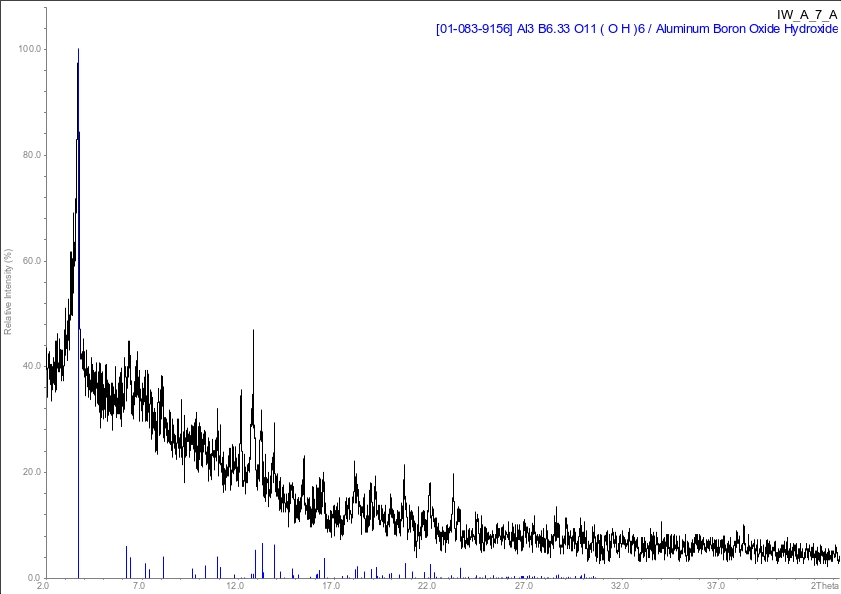
\includegraphics[height=8cm]{Images/AutoklaveA.jpeg}
    \caption{Diffraktogramm des Ansatzes A mit Vergleichswerten.}
    \label{fig:3}
\end{figure}

\noindent Das Diffraktogramm des Ansatz A lässt auf die Bildung der Vergleichsstruktur mit der Summenformel \ce{Al3B_{6.33}O11(OH)6} schließen, da prominente Reflexe des Produkts (schwarz) gut mit denen der Referenzstruktur (blau) übereinstimmen.

\begin{figure}[H]
    \centering
    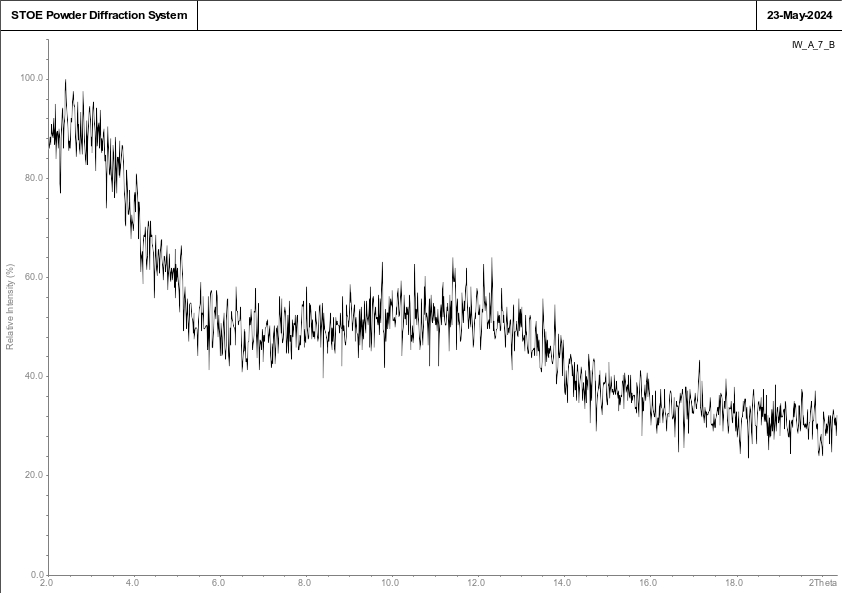
\includegraphics[height=8cm]{Images/AutoklaveB.jpeg}
    \caption{Diffraktogramm des Ansatzes B.}
    \label{fig:4}
\end{figure}

\noindent Das vermutlich amorphe Produkt des Ansatzes B führte zu einem Diffraktogramm, welches aufgrund starken Rauschens und Untergrunds nicht weiter ausgewertet werden konnte.

\begin{figure}[H]
    \centering
    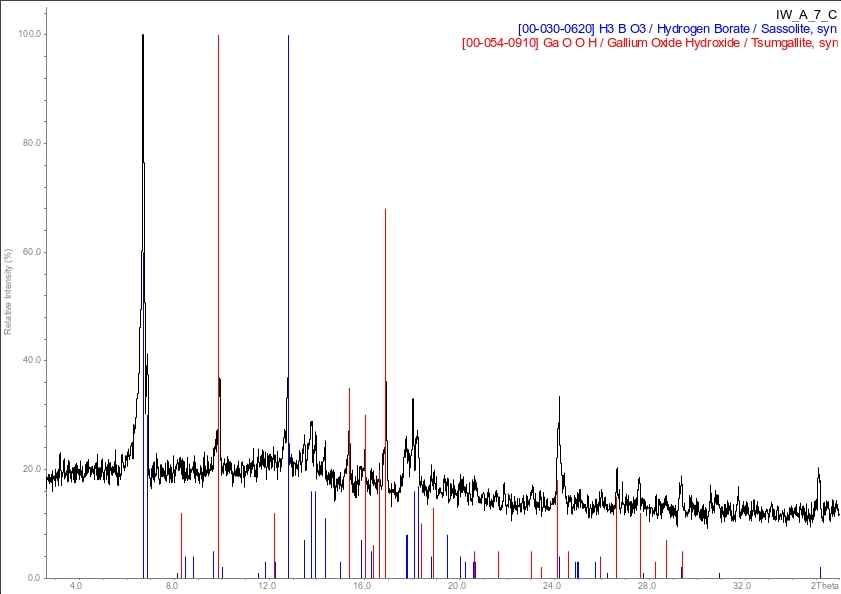
\includegraphics[height=8cm]{Images/AutoklaveC.jpeg}
    \caption{Diffraktogramm des Ansatzes C mit Vergleichswerten.}
    \label{fig:5}
\end{figure}

\noindent Das Produkt aus Ansatz C zeigt im Diffraktogramm (schwarz) charakteristische Reflexe für sowohl nicht reagierter Borsäure \ce{H3BO3} (blau) als auch für die der Referenz mit der Summenformel \ce{GaOOH} (rot).

\begin{figure}[H]
    \centering
    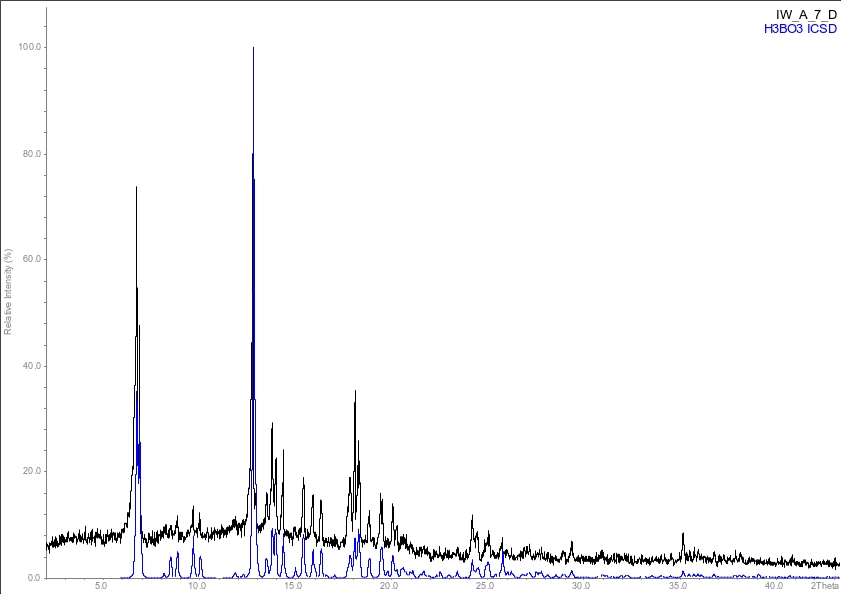
\includegraphics[height=8cm]{Images/AutoklaveD.jpeg}
    \caption{Diffraktogramm des Ansatzes D mit Vergleichswerten.}
    \label{fig:6}
\end{figure}

\noindent Die starke Präsenz der charakteristischen Borsäure Reflexe (blau) im Diffraktogramm des Ansatzes D (schwarz) lässt auf eine unvollständige Reaktion schließen.

\begin{figure}[H]
    \centering
    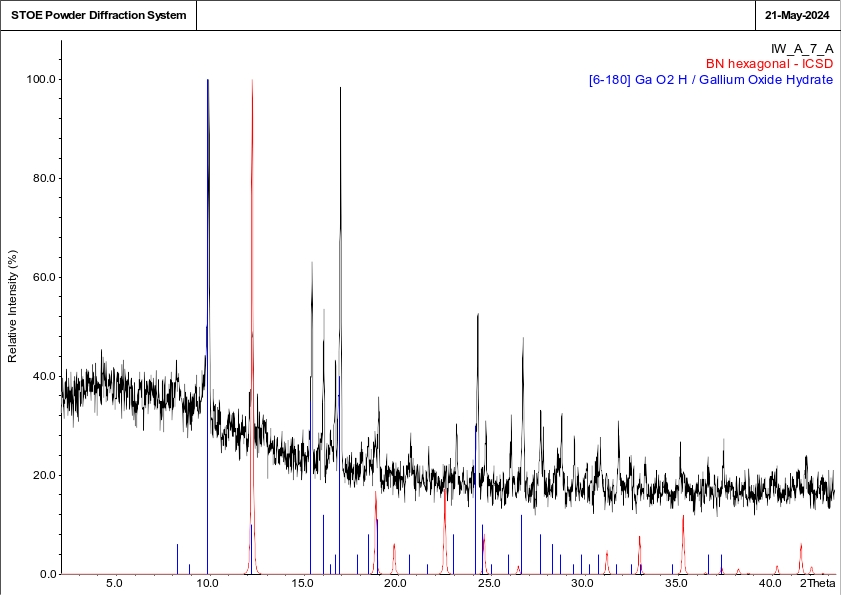
\includegraphics[height=8cm]{Images/AutoklaveE.jpeg}
    \caption{Diffraktogramm des Ansatzes E mit Vergleichswerten.}
    \label{fig:7}
\end{figure}

\noindent Erneut sind intensive Reflexe unreagierter Ausgangssubstanz, in diesem Fall Bornitrid \ce{BN} (rot), im Diffraktogramm des Ansatzes E (schwarz) erkennbar. 
Anders als im vorherigen Ansatz sind jedoch auch für die Referenzstruktur \ce{GaOOH} (blau) charakteristischen Peaks deutlich präsent, was auf eine zumindest in Teilen erfolgreiche Reaktion schließen lässt.


\selectlanguage{ngerman}
\bibliography{report}

\end{document}